%!TEX root = ../report.tex

\begin{document}
\chapter{Experimental Results}

\section{ Doored Areas }

\subsection { Door A }

Door A, is an excellent starting point and litmus test for various spatio-temporal
world modeling techniques due to its periodic, humanlike, and slightly random nature.
Door A's results establish a trend that can be seen
throughout the rest of the results. This is particularly visible in figure~\ref{figure:accuracy_door_A}
where the accuracy of each model is evaluated over time. Table~\ref{table:door_A}
also establishes a trend with respect to accuracy and computational resource
usage that is mirrored in the majority of experiments.\\

\begin{table}[h!]
  \centering
  \resizebox{\textwidth}{!}{%
    \begin{tabular}{|l|l|l|l|l|}
      \hline
      & DMM & Gaussian & FreMEn  & Hypertime \\ \hline
      Historical Accuracy             & 84.11\% & 77.80\%  & 92.51\% & 97.66\%   \\ \hline
      Prediction Accuracy             & 77.15\% & 79.43\%  & 87.08\% & 88.87\%   \\ \hline
      Computation Time (Milliseconds) & 610     & 50       & 70      & 5630      \\ \hline
      Memory Usage (KB)               & 31036   & 34968    & 34656   & 37192     \\ \hline
    \end{tabular}%
  }
  \caption{Door A Data Overview}
  \label{table:door_A}
\end{table}

Due to the periodic nature of the data, the techniques based off of extracting
periodicities (i.e. FreMEn and Hypertime) do an excellent job of recreating
past events as well as predicting future events. The prediction of past and future events can be seen in
figure~\ref{figure:historical_door_A} and~\ref{figure:future_door_A} respectively. HyperTime's slightly better
prediction ability is most likely due to the extra steps taken to wrap the data back
in on itself temporally. However, this additional training and accuracy comes at a
great cost. Hypertime manages only a small performance increase of
around one percent over FreMEn with the total training and prediction time
taking on the order of two magnitudes longer when compared to either Gaussian or FreMEn.
Finally, it appears that the Gaussian model completely failed to predict any
open state. This is likely due to the sparseness of positive, or open
states resulting in the model oscillating between 0 and just under 0.5 thus
never reaching the open threshold. \\

\begin{center}
  \begin{figure}[!Hp]
  \begin{tabular}{cc}
    {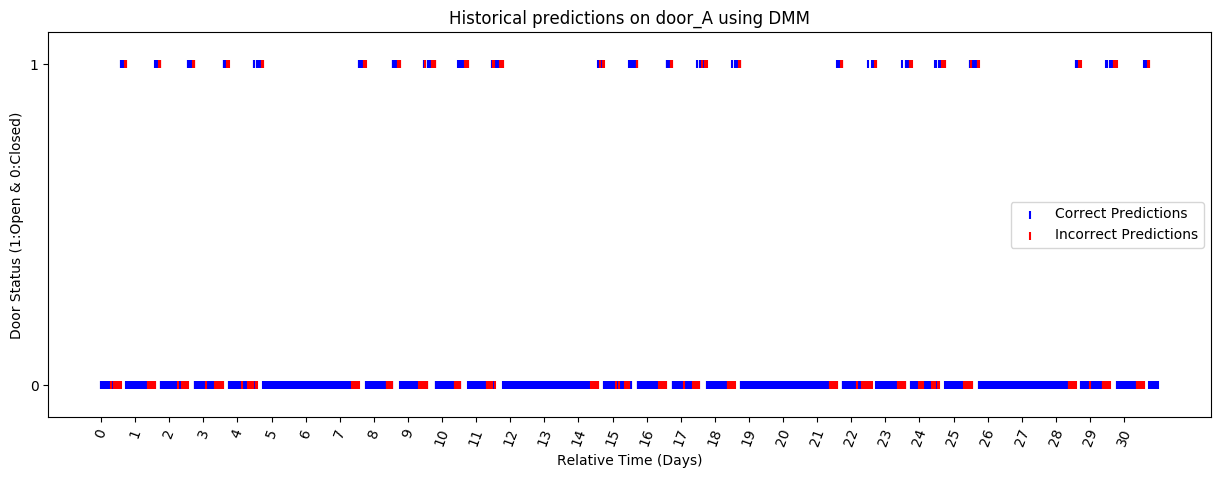
\includegraphics[width = 6in]{images/results/Historical_door_A_DMM.png}} \\
    {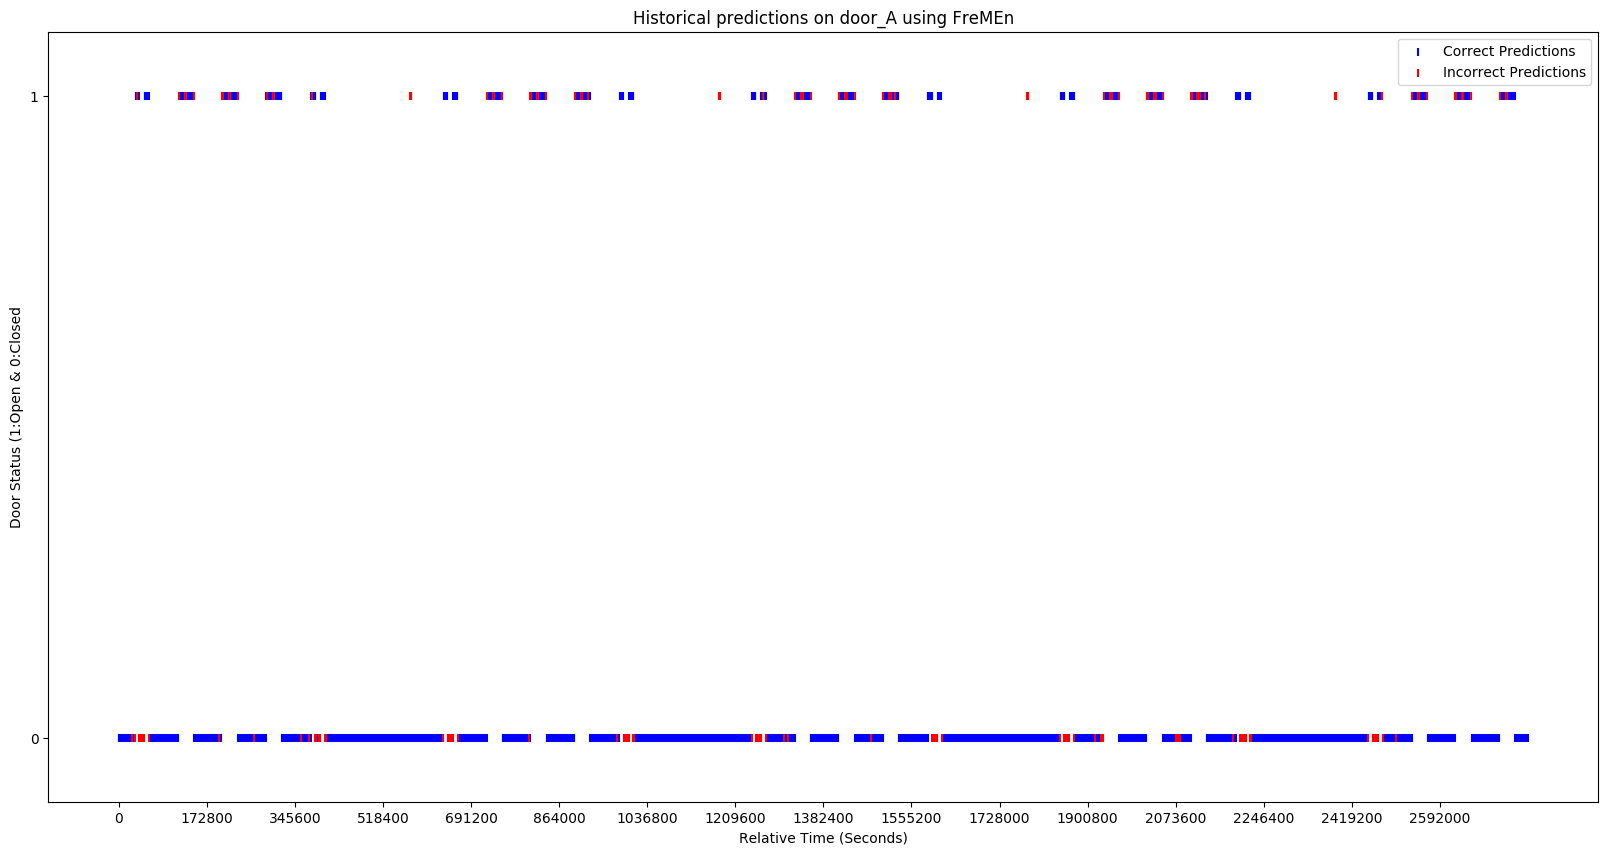
\includegraphics[width = 6in]{images/results/Historical_door_A_FreMEn.png}} \\
    {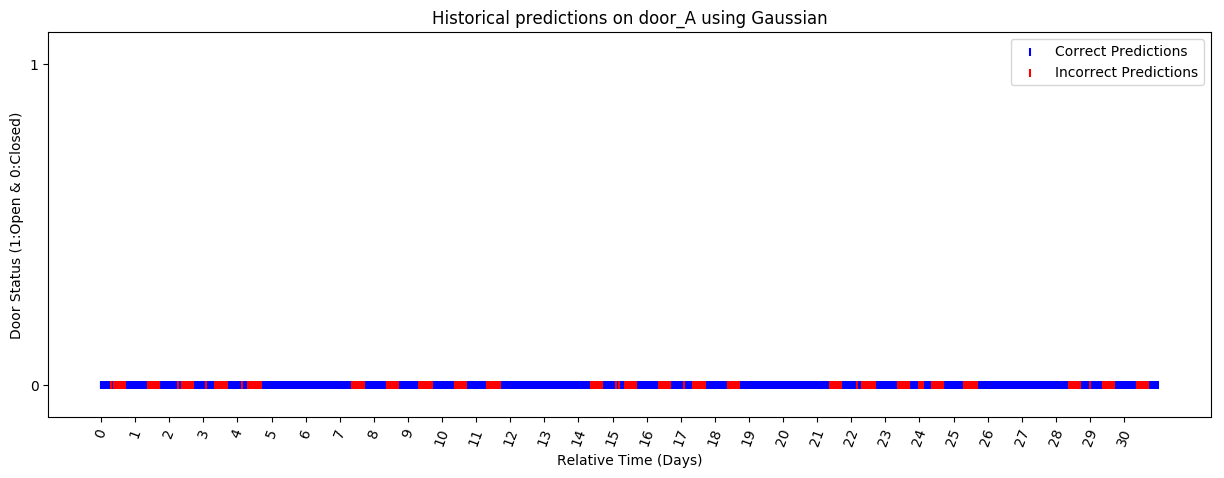
\includegraphics[width = 6in]{images/results/Historical_door_A_Gaussian.png}} \\
    {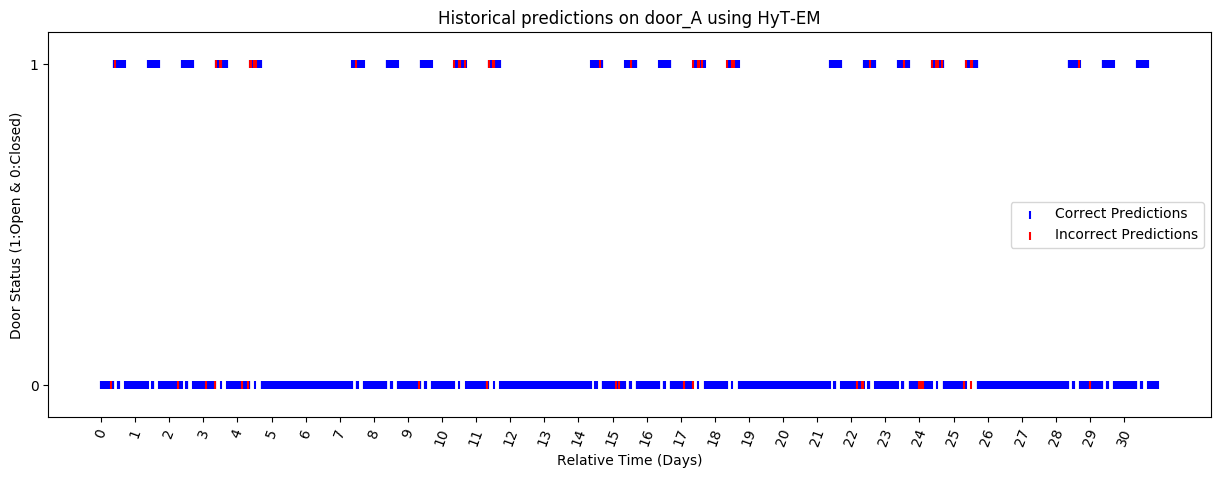
\includegraphics[width = 6in]{images/results/Historical_door_A_HyT-EM.png}} \\
  \end{tabular}
  \caption{Historical Recreations - Door A}
  \label{figure:historical_door_A}
\end{figure} \\ \\

\begin{figure}[!Hp]
  \begin{tabular}{cc}
    {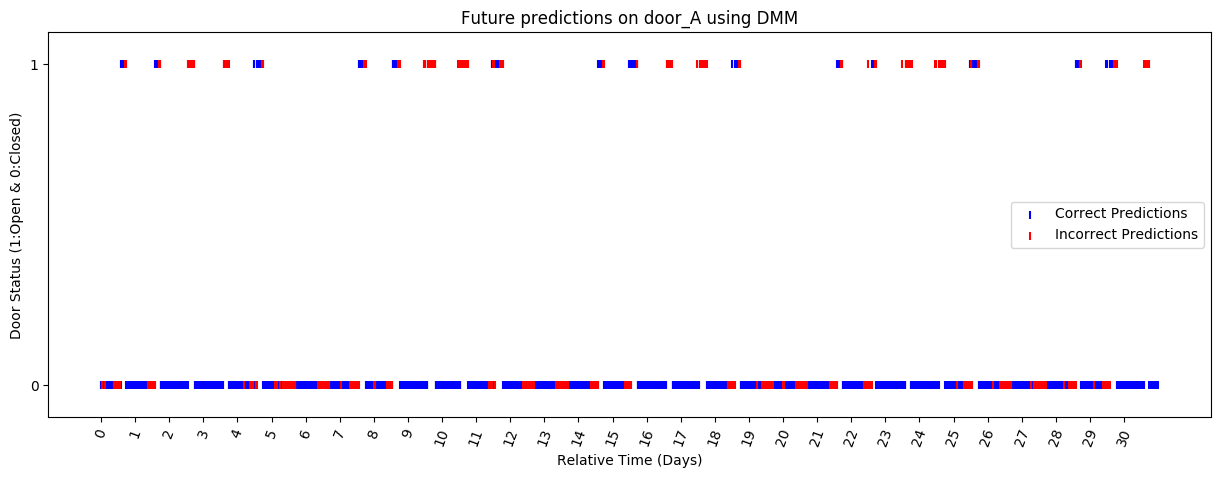
\includegraphics[width = 6in]{images/results/Future_door_A_DMM.png}} \\
    {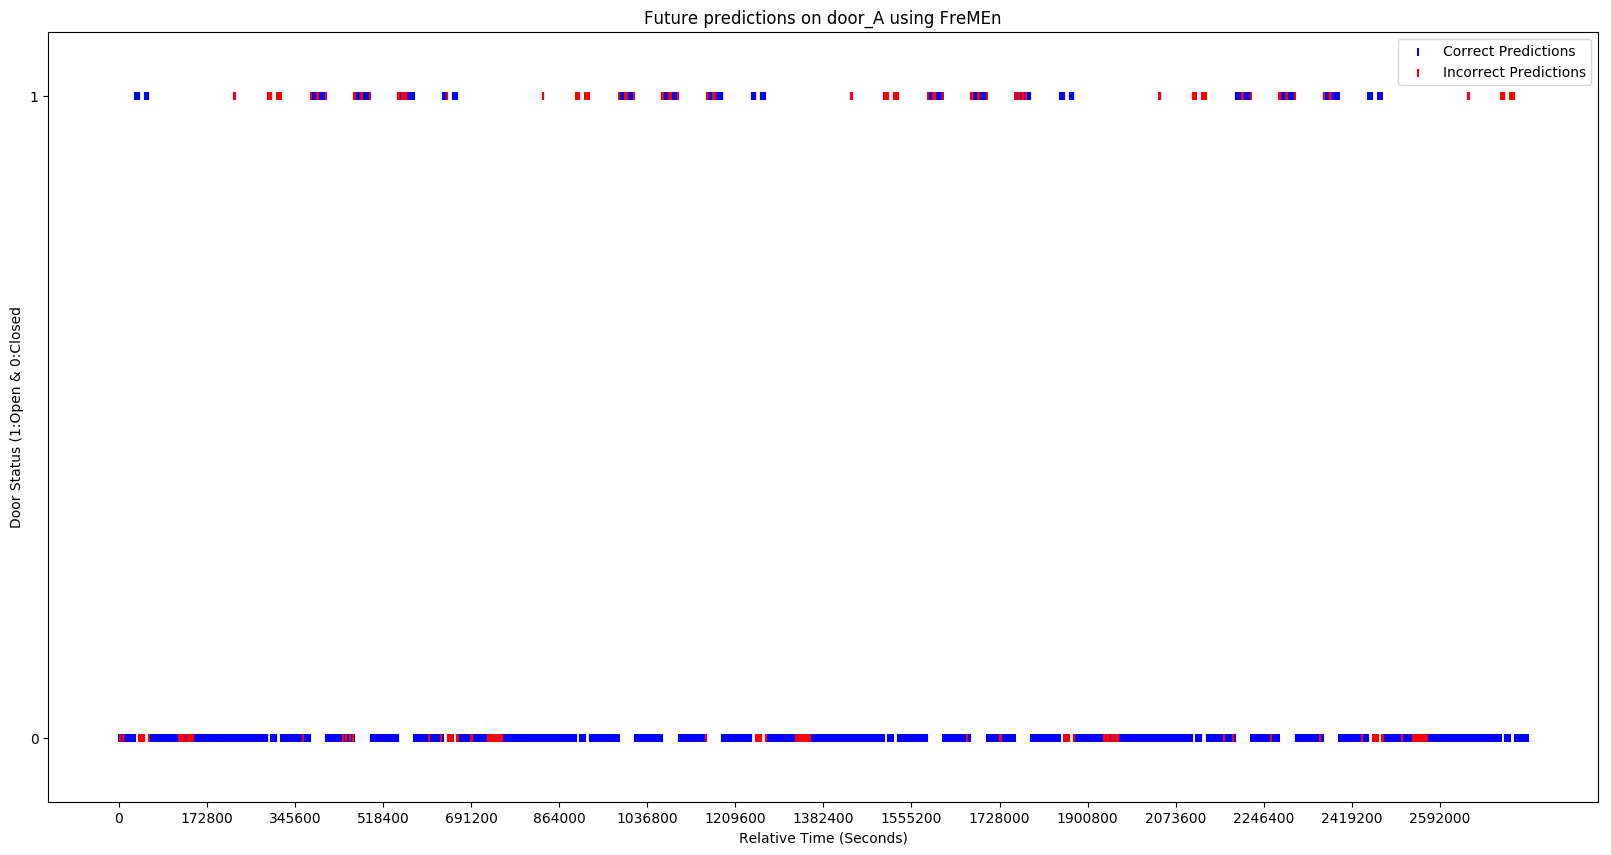
\includegraphics[width = 6in]{images/results/Future_door_A_FreMEn.png}} \\
    {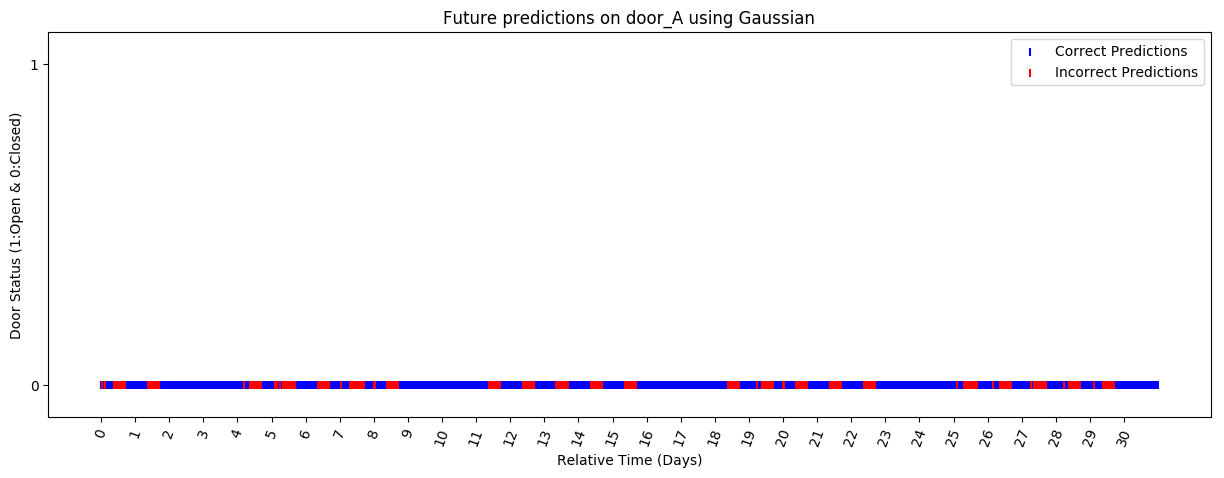
\includegraphics[width = 6in]{images/results/Future_door_A_Gaussian.png}} \\
    {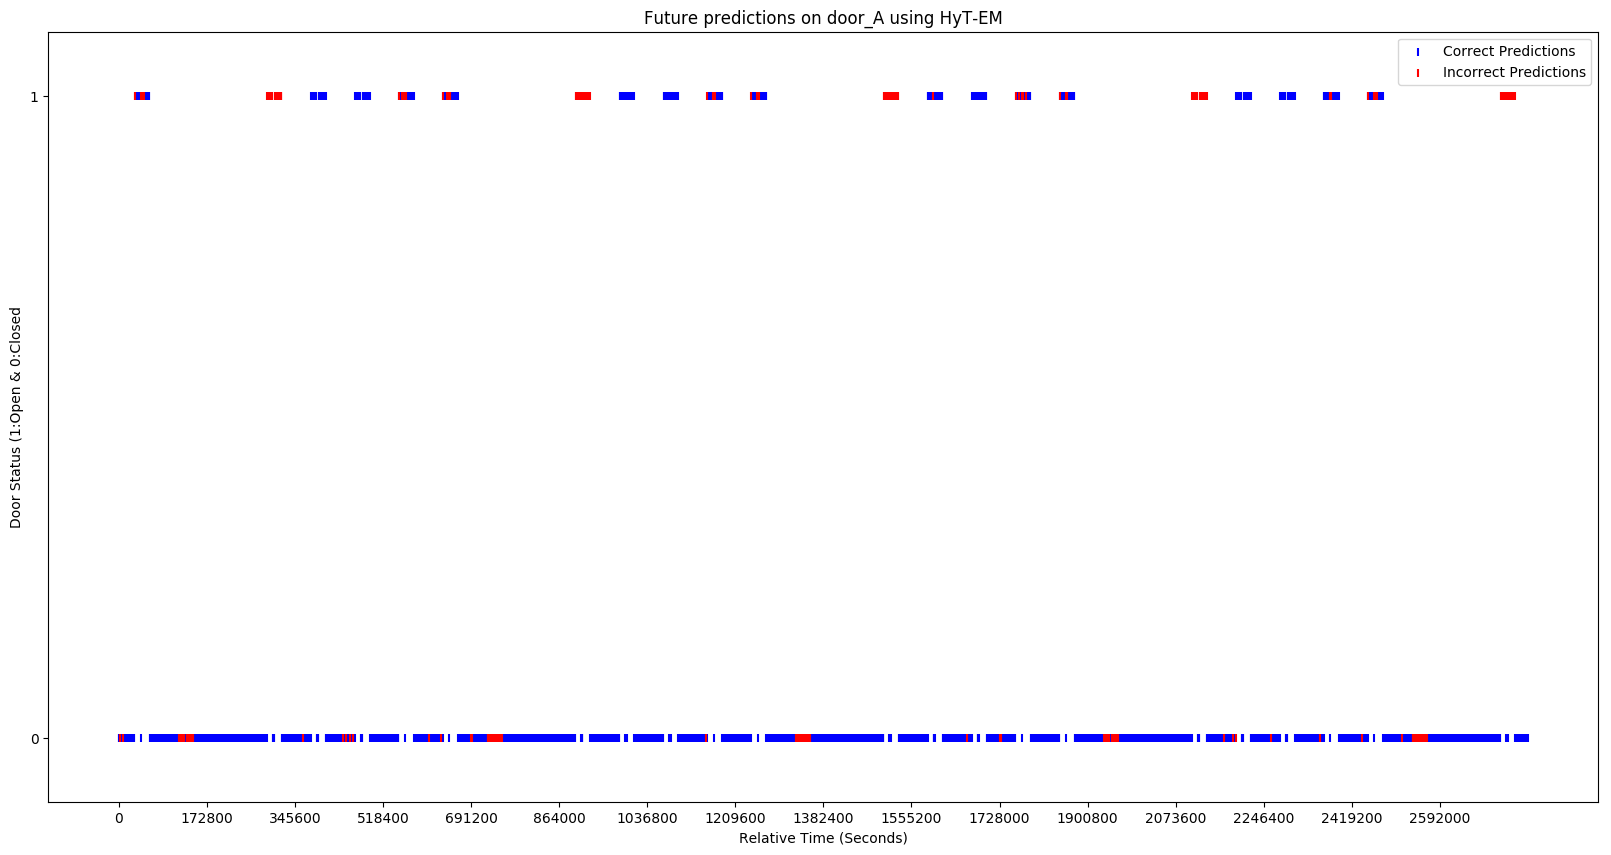
\includegraphics[width = 6in]{images/results/Future_door_A_HyT-EM.png}} \\
  \end{tabular}
  \caption{Future Predictions - Door A}
  \label{figure:future_door_A}
\end{figure} \\ \\

\begin{figure}[!Hp]
  \begin{tabular}{cc}
    {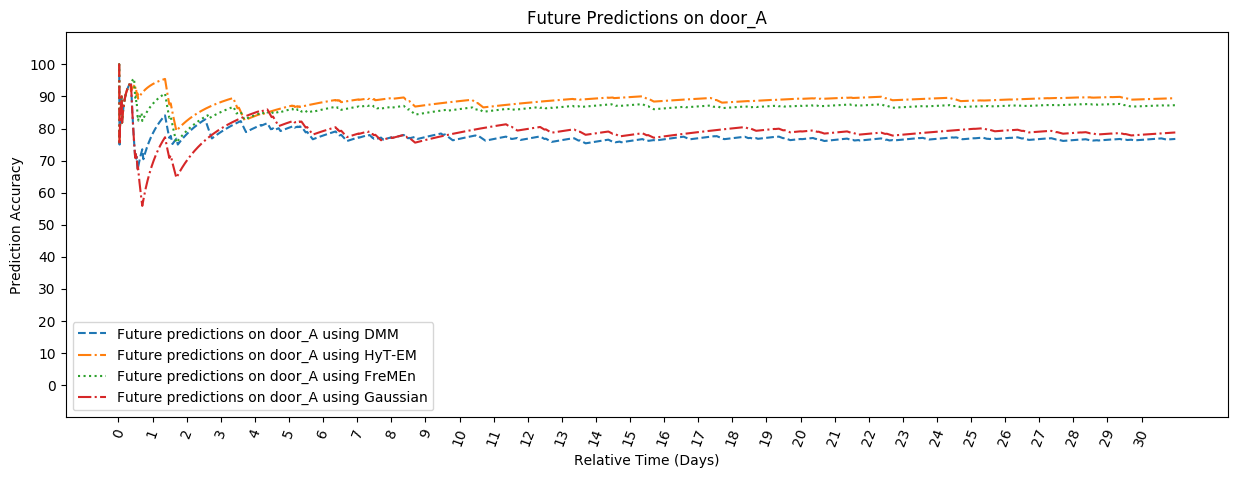
\includegraphics[width = 6in]{images/results/Future_Predictions_on_door_A.png}} \\
    {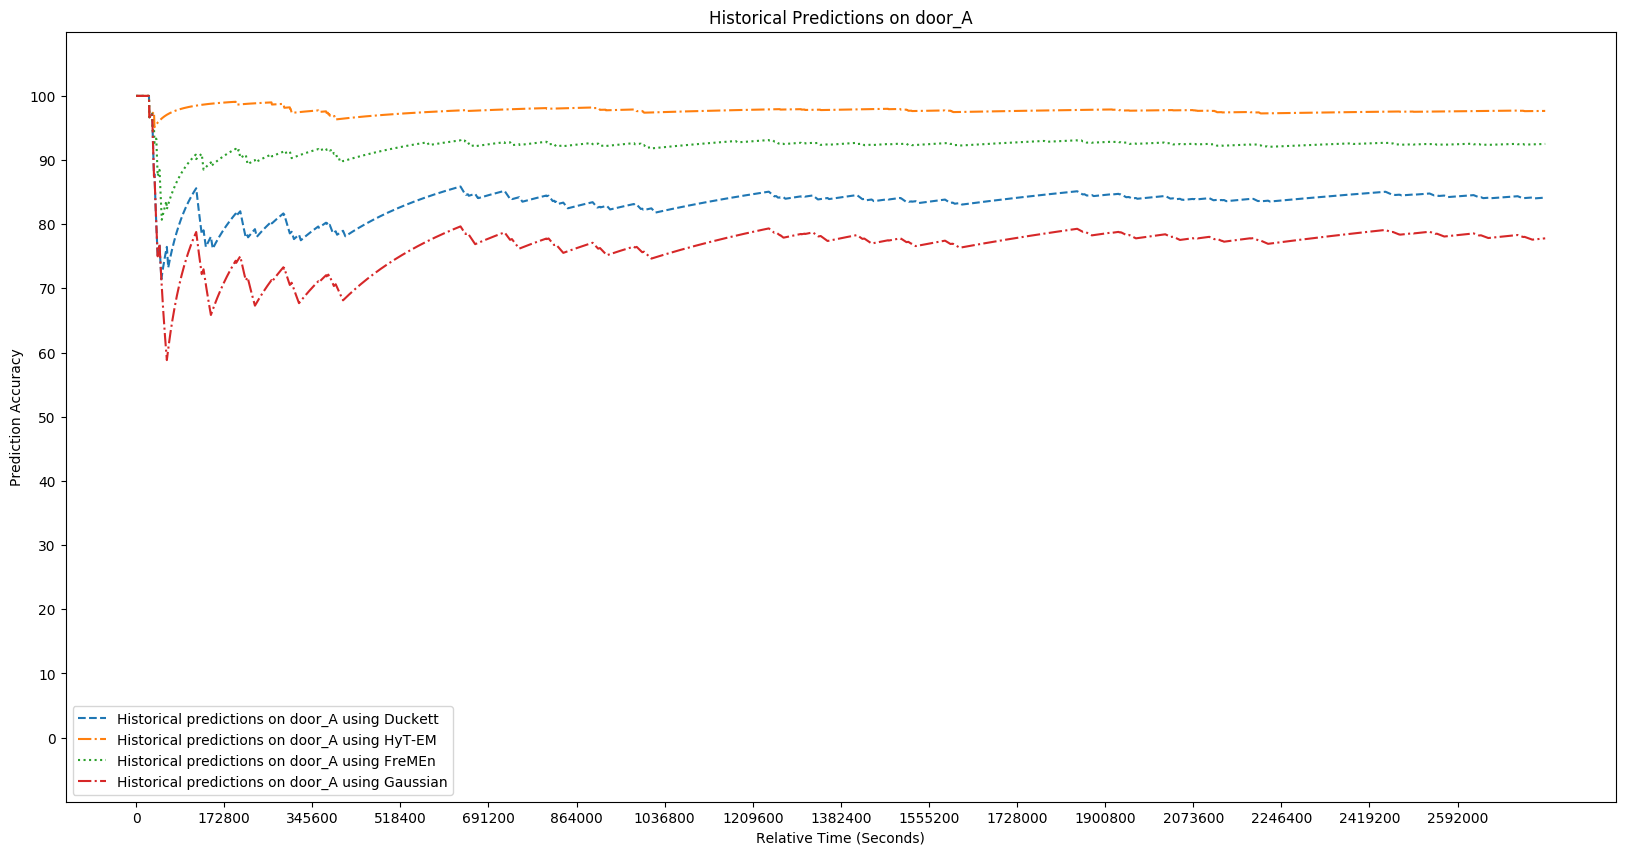
\includegraphics[width = 6in]{images/results/Historical_Predictions_on_door_A.png}} \\
  \end{tabular}
  \caption{Model Accuracy Over Time - Door A}
  \label{figure:accuracy_door_A}
\end{figure} \\ \\
\end{center}

\subsection { Door B }

Door B demonstrates a fact the will be come increasingly clear with future
experiments. Methods that use a modified version of the Fourier transform as
described in \cite{Krajnik2015} require a certain threshold of frequency to be met
in order to accurately make predictions. In fact, its interesting to note that the
very thing that allows these methods perform so well with periodic behavior
causes issues within datasets with non periodic behavior or datasets with
minimal periods of periodic data. \\

\begin{table}[h!]
  \centering
  \resizebox{\textwidth}{!}{%
    \begin{tabular}{|l|l|l|l|l|}
      \hline
      & DMM & Gaussian & FreMEn  & Hypertime \\ \hline
      Historical Accuracy             & 85.71\% & 59.81\%  & 75.20\% & 71.55\%   \\ \hline
      Prediction Accuracy             & 69.24\% & 62.17\%  & 76.95\% & 75.78\%   \\ \hline
      Computation Time (Milliseconds) & 600     & 60       & 80      & 1440      \\ \hline
      Memory Usage (KB)               & 31036   & 34644    & 34892   & 37692     \\ \hline
    \end{tabular}%
  }
  \caption{Door B Data Overview}
  \label{table:door_B}
\end{table} \\

DMM, relying almost solely on averages, does surprisingly well in this
experiment, beating all other models in both historical and prediction
accuracy visible in figure~\ref{figure:historical_door_B} and~\ref{figure:future_door_B}. It is, however, important to note the flaws in DMM's long-term
prediction. Due to the fact that future predictions are not directly possible
using DMM and thus historical data is used, it is clear that,
while DMM performed well overall historically, it is not without problems
in future prediction. Of particular interest is DMM's failure to continue to
accurately predict a periodic behavior that does not occur on month
boundaries. Since the behavior that happens every three days does not happen
on the same day between the two months DMM incorrectly predicts its
occurrence as happening on the same days each month. \\

In terms of resource usage, a similar trend to door A is observed as visible
in~\ref{table:door_B}. Gaussian
and FreMEn predictions take under 100 milliseconds while DMM takes around
an order of magnitude longer, and Hypertime yet another order of magnitude
beyond that. Finally, again, similar to door A, all approaches use roughly the same amount
of memory for training and predicting at around 30 megabytes and
within about 10 megabytes of one another. \\

\begin{center}
\begin{figure}[!Hp]
  \begin{tabular}{cc}
    {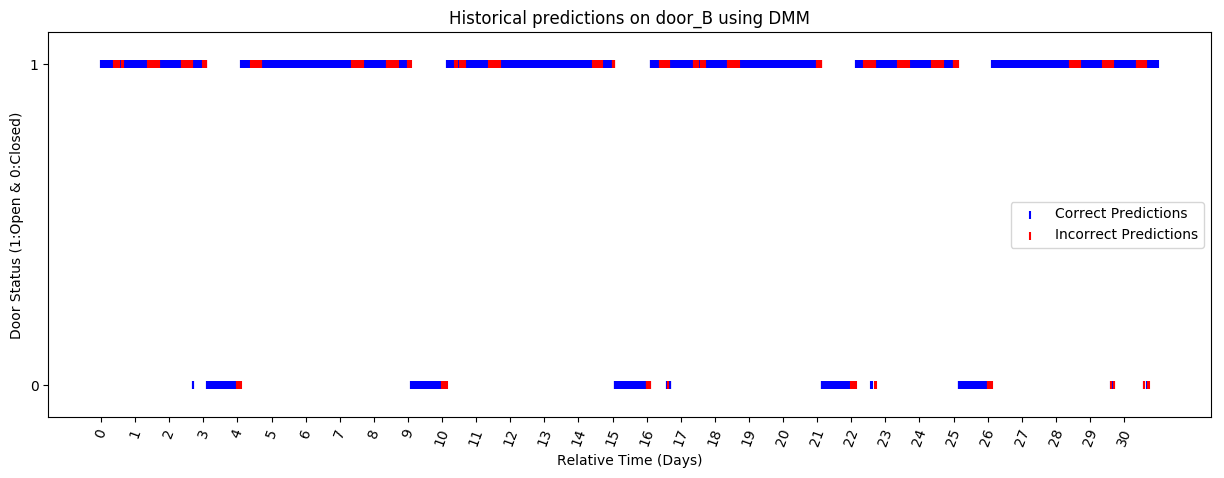
\includegraphics[width = 6in]{images/results/Historical_door_B_DMM.png}} \\
    {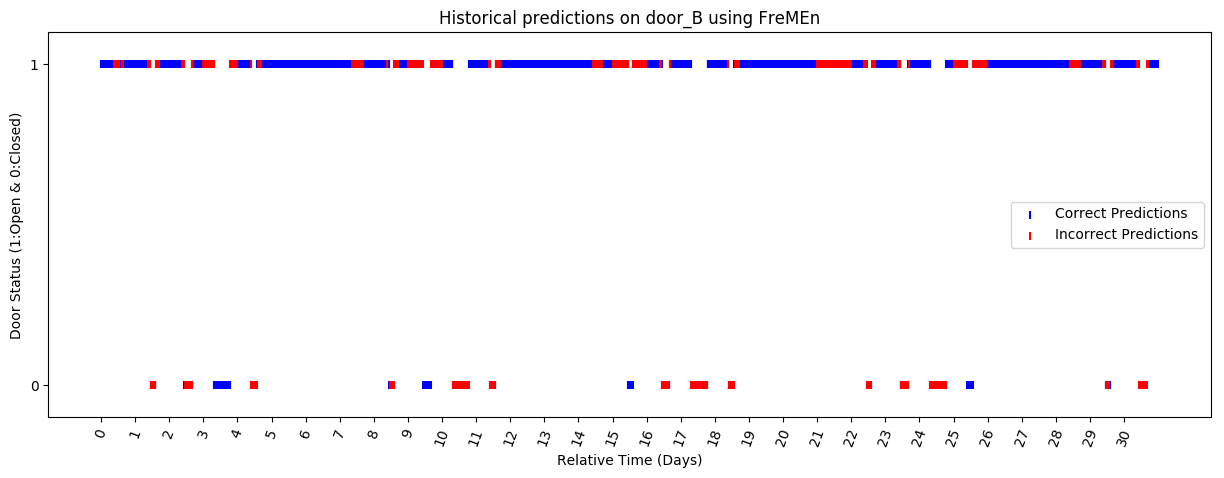
\includegraphics[width = 6in]{images/results/Historical_door_B_FreMEn.png}} \\
    {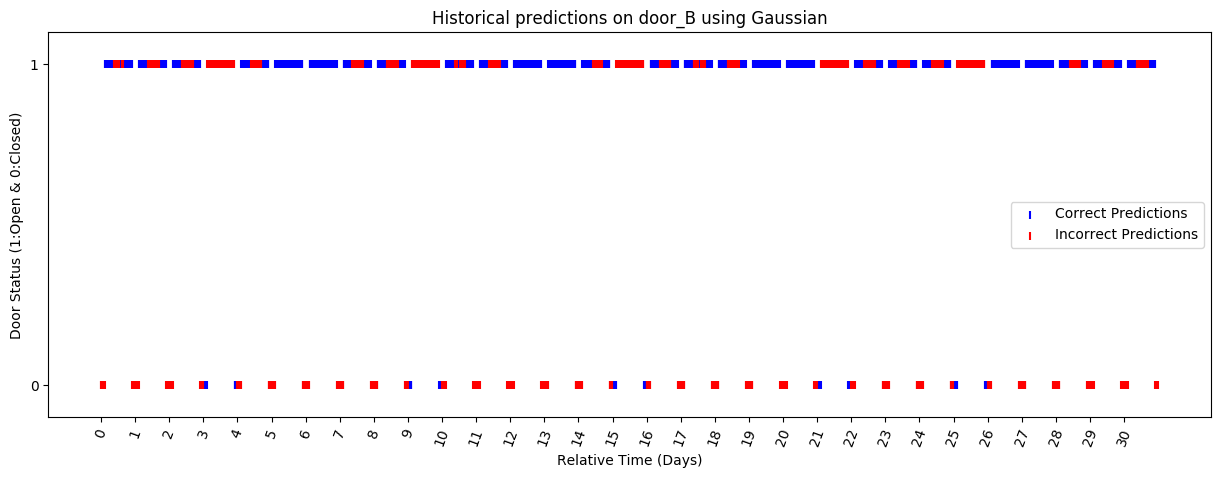
\includegraphics[width = 6in]{images/results/Historical_door_B_Gaussian.png}} \\
    {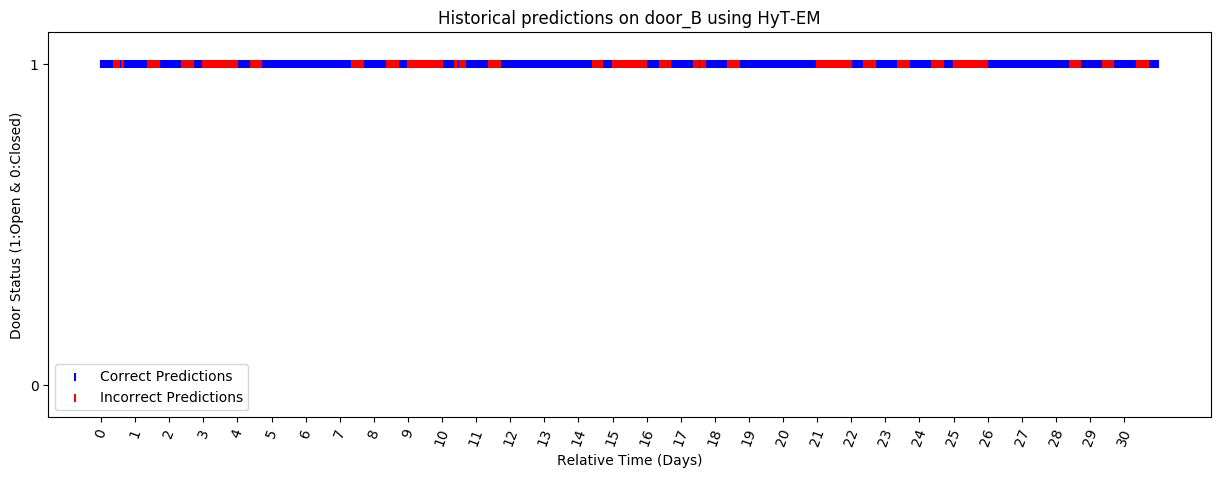
\includegraphics[width = 6in]{images/results/Historical_door_B_HyT-EM.png}} \\
  \end{tabular}
  \caption{Historical Recreations - Door B}
  \label{figure:historical_door_B}
\end{figure}\\ \\

\begin{figure}[!Hp]
  \begin{tabular}{cc}
    {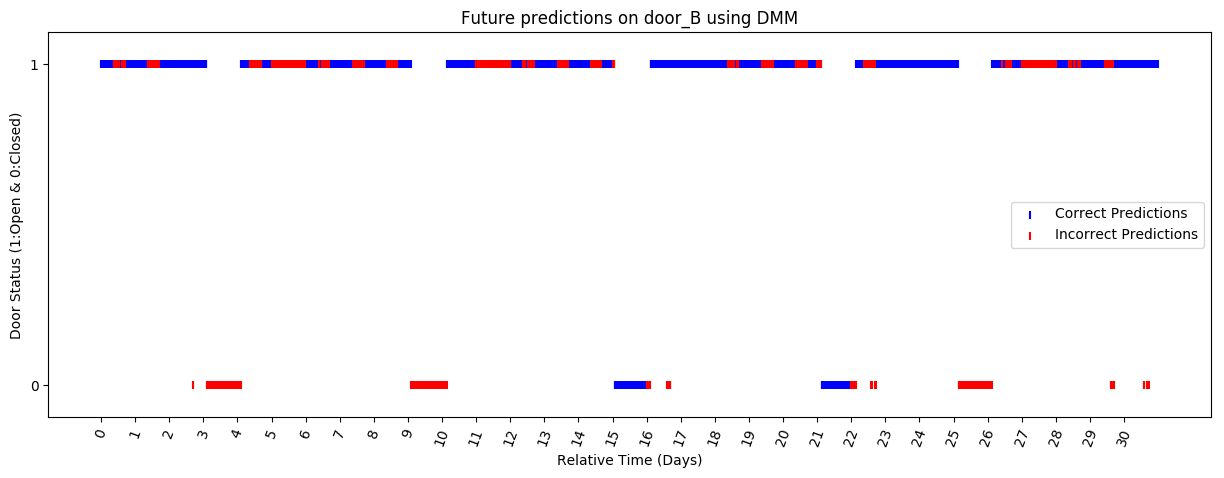
\includegraphics[width = 6in]{images/results/Future_door_B_DMM.png}} \\
    {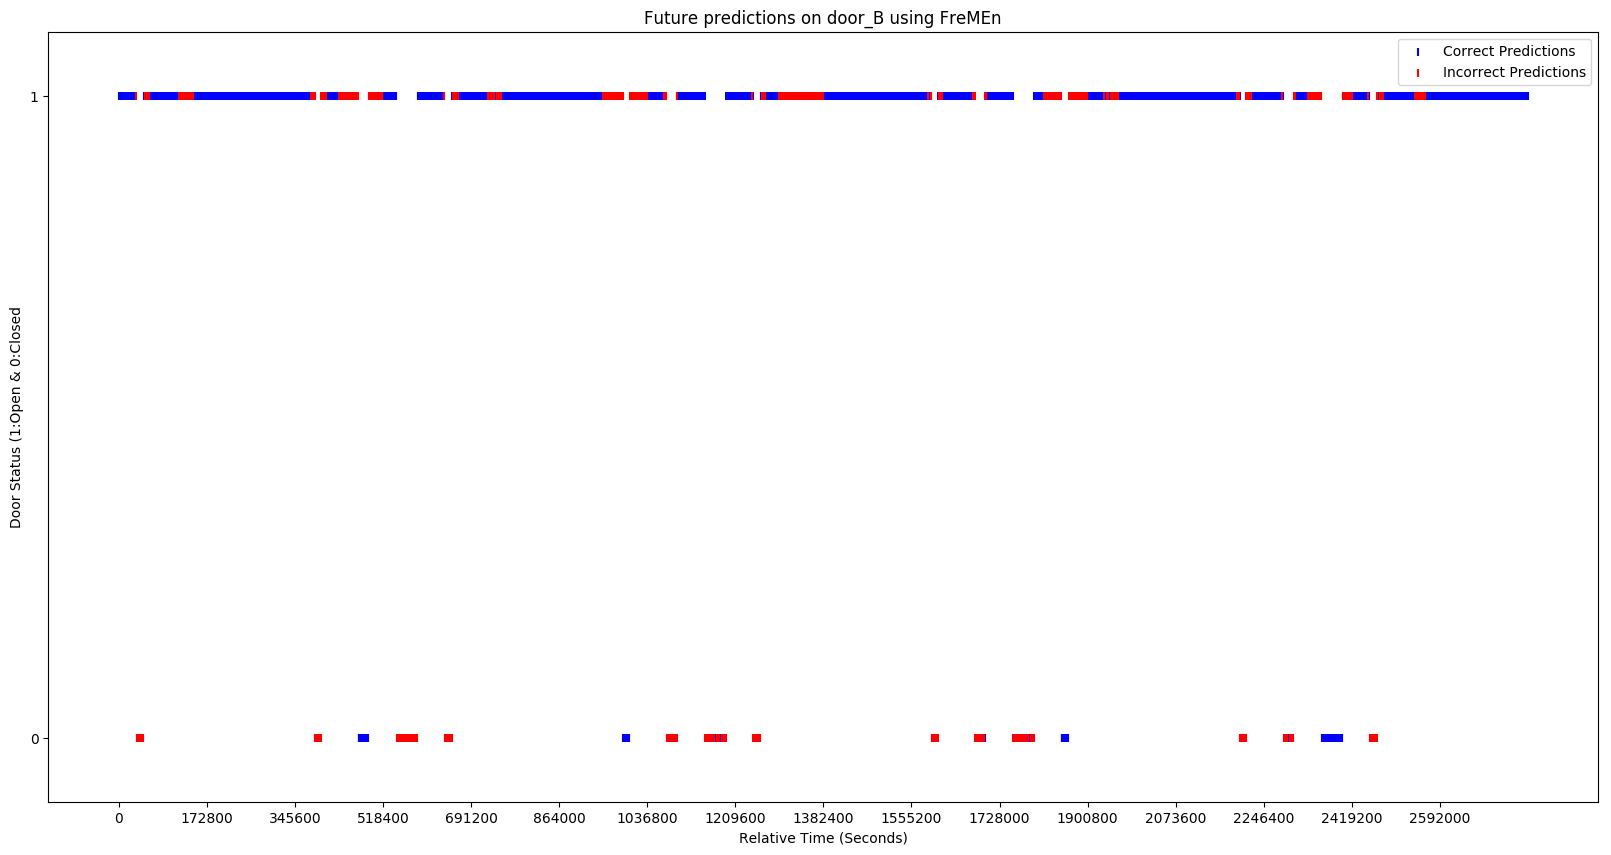
\includegraphics[width = 6in]{images/results/Future_door_B_FreMEn.png}} \\
    {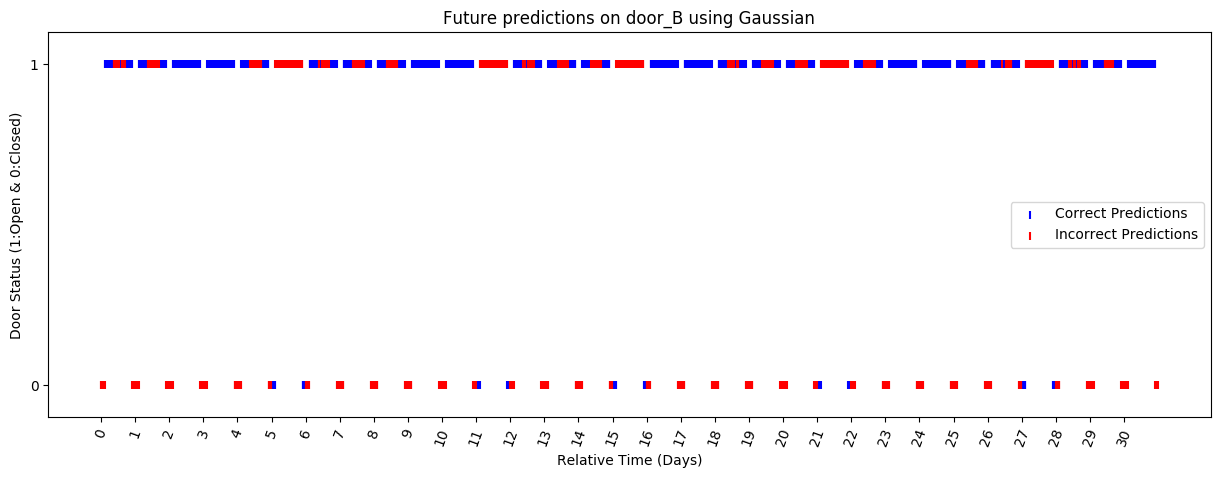
\includegraphics[width = 6in]{images/results/Future_door_B_Gaussian.png}} \\
    {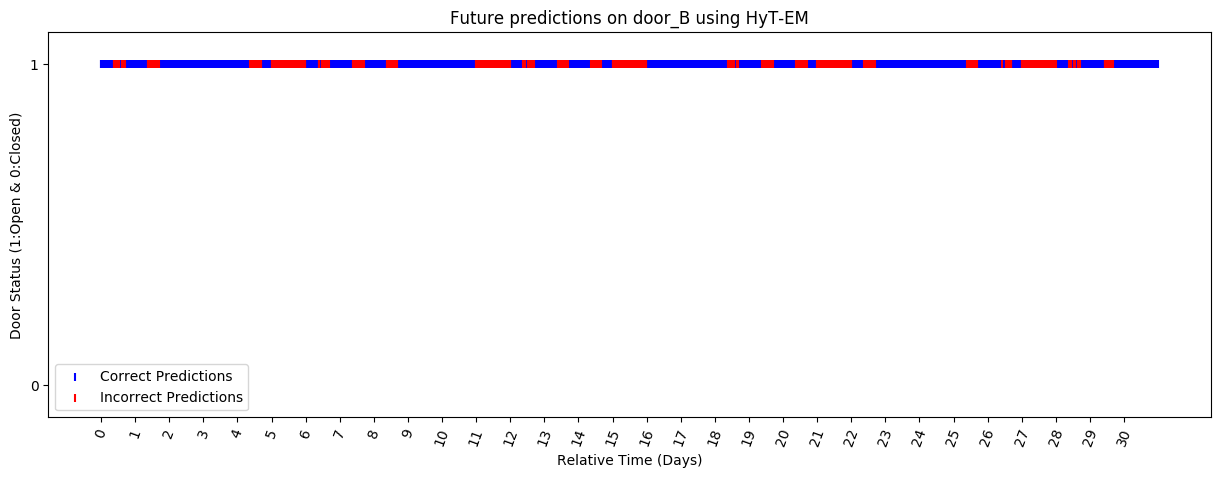
\includegraphics[width = 6in]{images/results/Future_door_B_HyT-EM.png}} \\
  \end{tabular}
  \caption{Future Predictions - Door B}
  \label{figure:future_door_B}
\end{figure}\\ \\

\begin{figure}[!Hp]
  \begin{tabular}{cc}
    {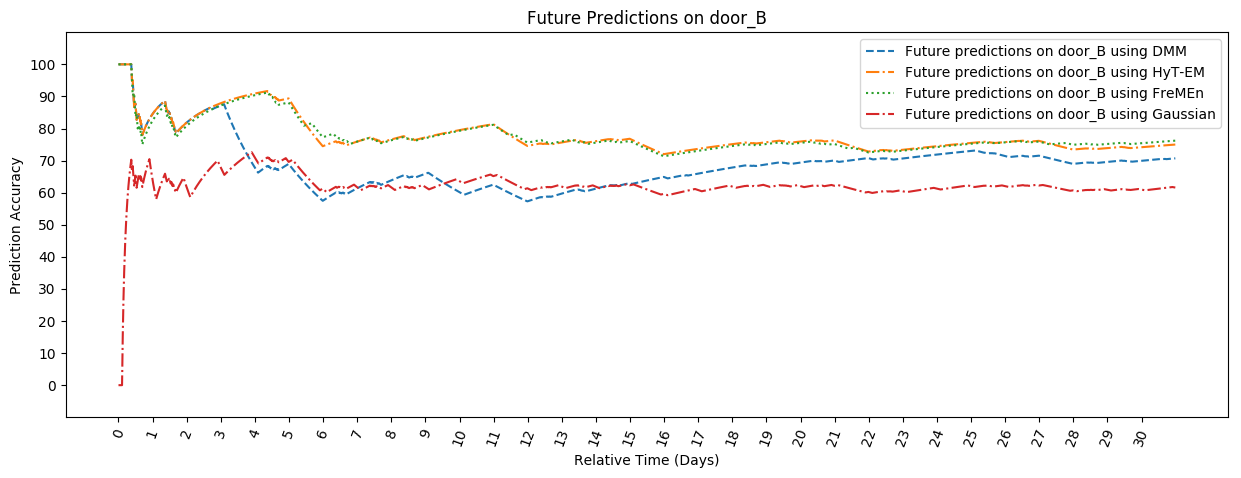
\includegraphics[width = 6in]{images/results/Future_Predictions_on_door_B.png}} \\
    {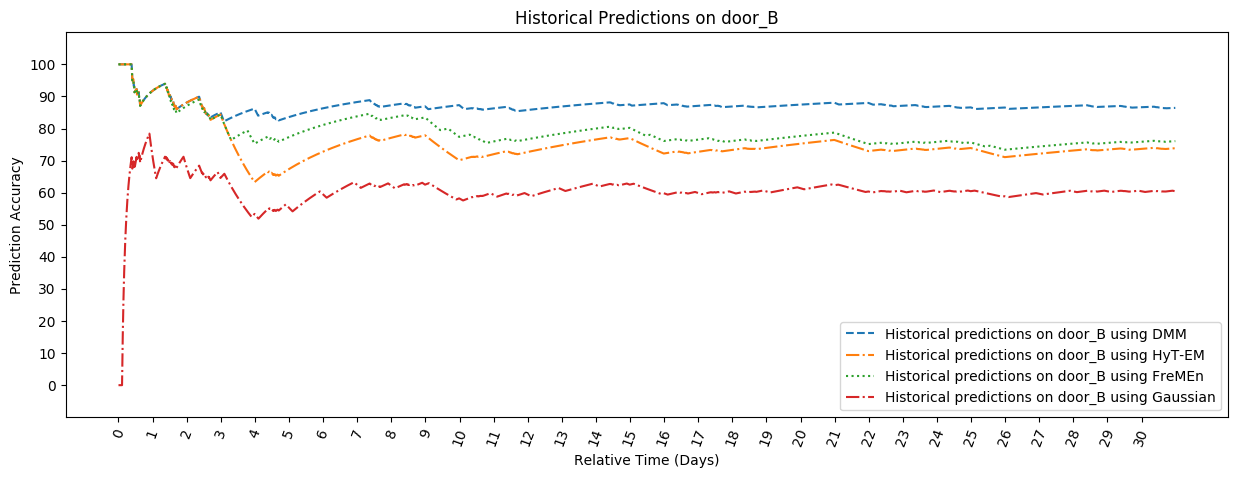
\includegraphics[width = 6in]{images/results/Historical_Predictions_on_door_B.png}} \\
  \end{tabular}
  \caption{Model Accuracy Over Time - Door B}
  \label{figure:accuracy_door_B}
\end{figure}\\ \\
\end{center}


\subsection { Door C }

With door A exemplifying the occasionally periodic and somewhat noisy
behaviour in the real-world, door C serves as almost the exact opposite,
modeling a one time, long-term change.
Perhaps expectedly, the results in terms of prediction accuracy are
almost completely opposite to that of door A with DMM having the best
performance both historically and with future predictions. \\

Unfortunately, despite DMM's better performance by the numbers in table
~\ref{table:door_C}
looking at the resulting graphs in figures
~\ref{figure:historical_door_C} and~\ref{figure:future_door_C}
show a somewhat
initially disappointing result. As discussed in the door B experiment,
DMM, merely uses its historical predictions again for future
predictions. This is clearly visible by the prediction of door C being open
for the first three weeks in the future predictions. However, DMM was not
designed for long-term future predictions and is instead meant to be used
``live''. When this is accounted for, DMM's performance is once again
impressive. In fact, as mentioned in the previous section the
historical predictions made by DMM can be viewed as it's ``live''
predictions and thus it would be expected that in the real-world it would
continue to predict the door as being closed as long as long-term future
predictions are not requested. Thus it is likely that DMM's
performance would be closer to 100\% for future actives for as long as the door
remained shut. \\

\begin{table}[h!]
  \centering
  \resizebox{\textwidth}{!}{%
    \begin{tabular}{|l|l|l|l|l|}
      \hline
      & DMM & Gaussian & FreMEn  & Hypertime \\ \hline
      Historical Accuracy             & 99.56\% & 62.75\%  & 67.74\% & 67.74\%   \\ \hline
      Prediction Accuracy             & 31.82\% & 14.58\%  & 00.00\% & 00.00\%   \\ \hline
      Computation Time (Milliseconds) & 570     & 60       & 70      & 530       \\ \hline
      Memory Usage (KB)               & 31224   & 35004    & 34976   & 37208     \\ \hline
    \end{tabular}%
  }
  \caption{Door C Data Overview}
  \label{table:door_C}
\end{table}

As alluded to above in door B's experiment, the lack of periodic data has
caused both FreMEn and Hypertime to take the easiest prediction for the
training data and predict that the door will always be open. Unfortunately,
this causes the future predictions, seen in figure~\ref{figure:future_door_C} to be entirely inaccurate. The only possible redemption
for the Fourier based approaches on this long-term change is that the
prediction would eventually flip to always being closed, but only after the total number of observations of the door being
closed surpassed that of the door being open. In this case, that would take a
total of just over 6 weeks if training was being done every night. \\

The resource usage statistics in table~\ref{table:door_C} do interestingly break slightly
from the norm. It appears that due to the simplistic predictions of the
Fourier approaches, Hypertime has shaved off an order of magnitude in
computation time. This is believed to be because the prediction model created
by Hypertime, after the initial naive approach, has a larger error than the first and thus it immediately quits
and stops attempting to improve the model. This is irrelevant however, seeing
as the predictions are completely inaccurate so any gain in computational time
is meaningless as seen in figure~\ref{figure:accuracy_door_C}\\

\begin{center}
\begin{figure}[!Hp]
  \begin{tabular}{cc}
    {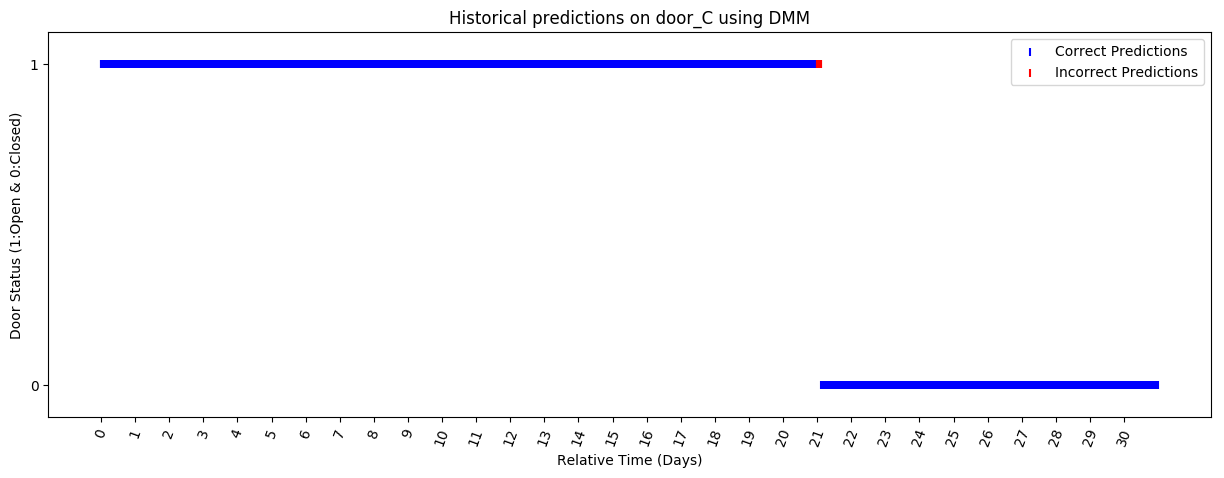
\includegraphics[width = 6in]{images/results/Historical_door_C_DMM.png}} \\
    {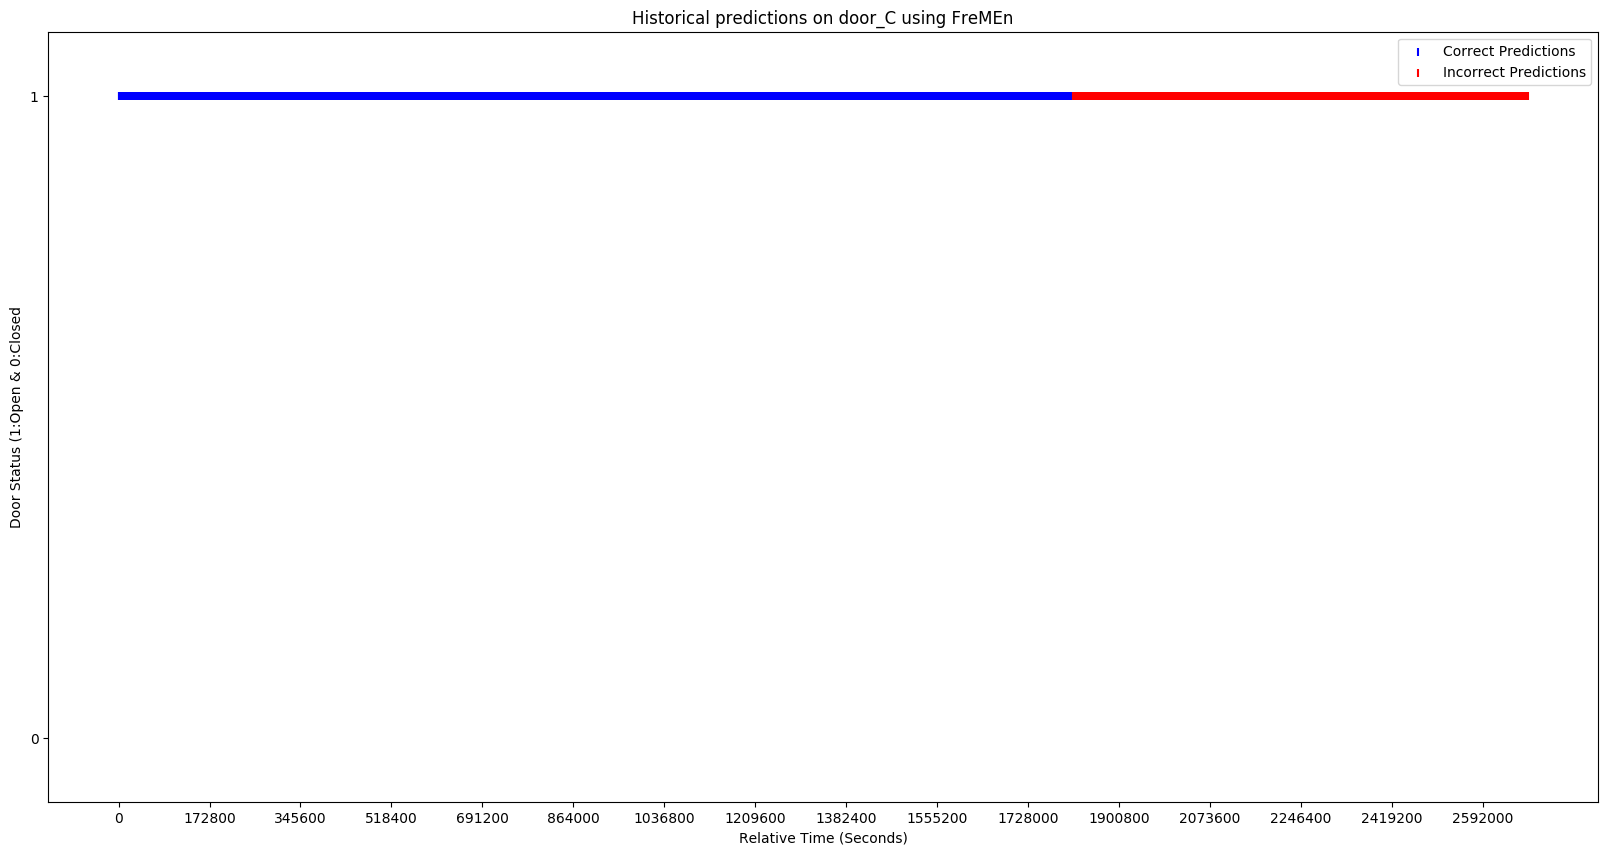
\includegraphics[width = 6in]{images/results/Historical_door_C_FreMEn.png}} \\
    {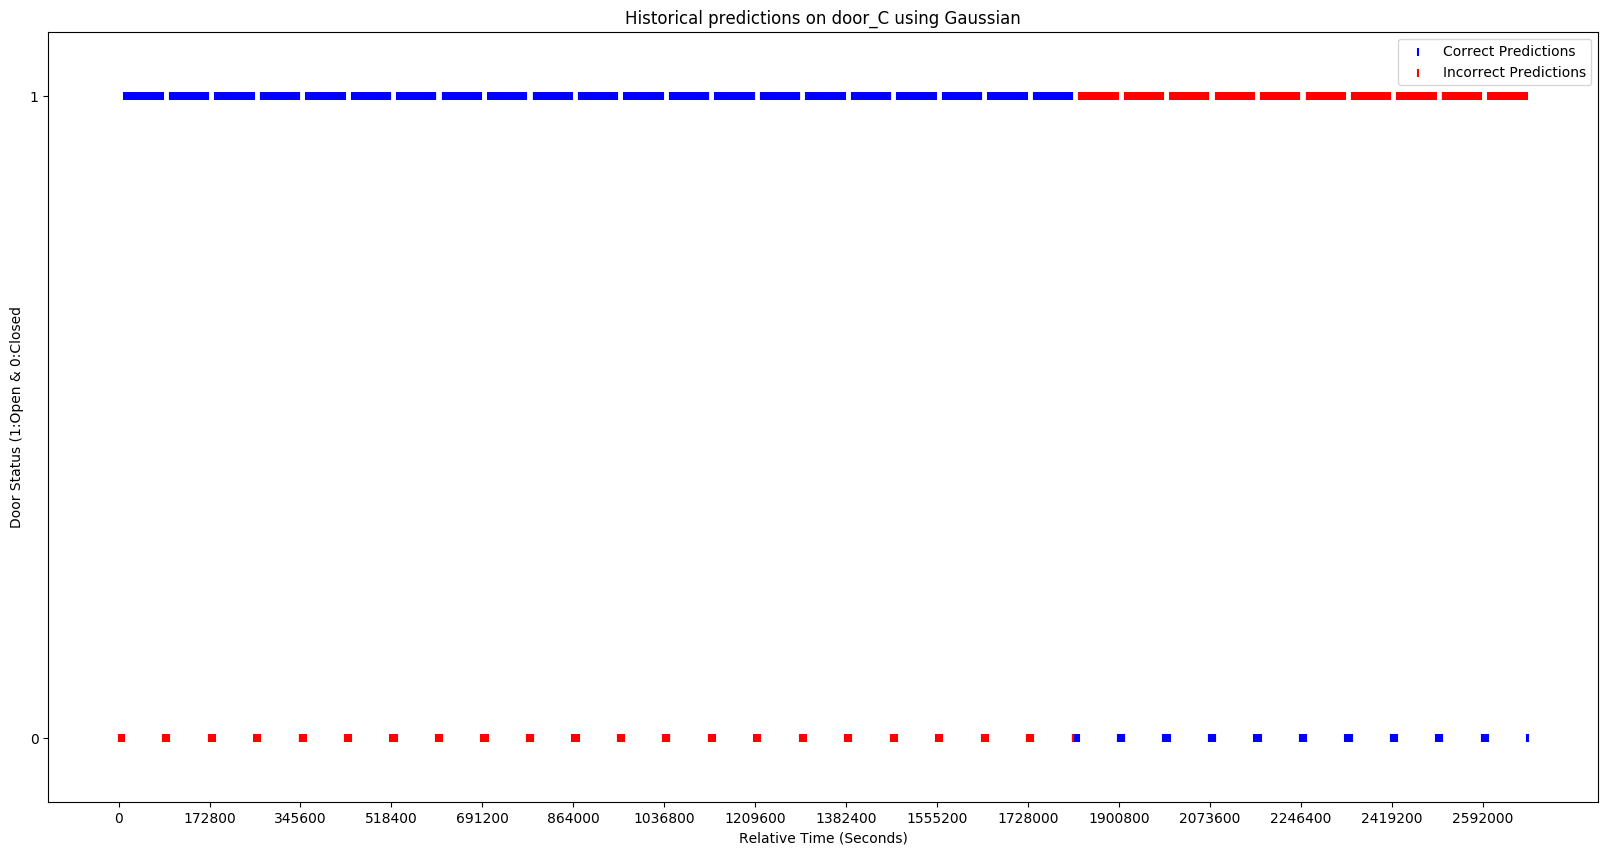
\includegraphics[width = 6in]{images/results/Historical_door_C_Gaussian.png}} \\
    {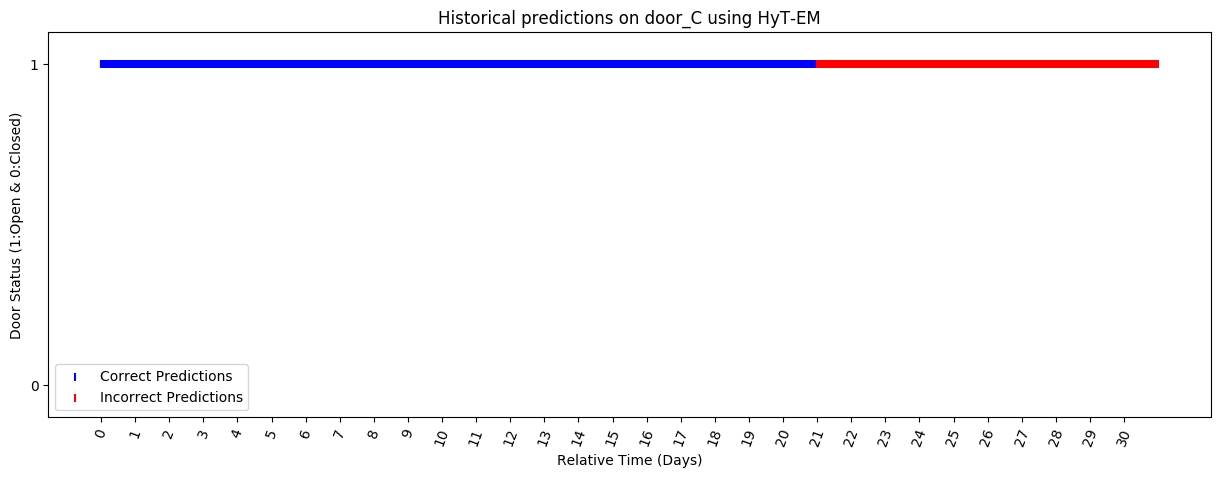
\includegraphics[width = 6in]{images/results/Historical_door_C_HyT-EM.png}} \\
  \end{tabular}
  \caption{Historical Recreations - Door C}
  \label{figure:historical_door_C}
\end{figure}\\ \\

\begin{figure}[!Hp]
  \begin{tabular}{cc}
    {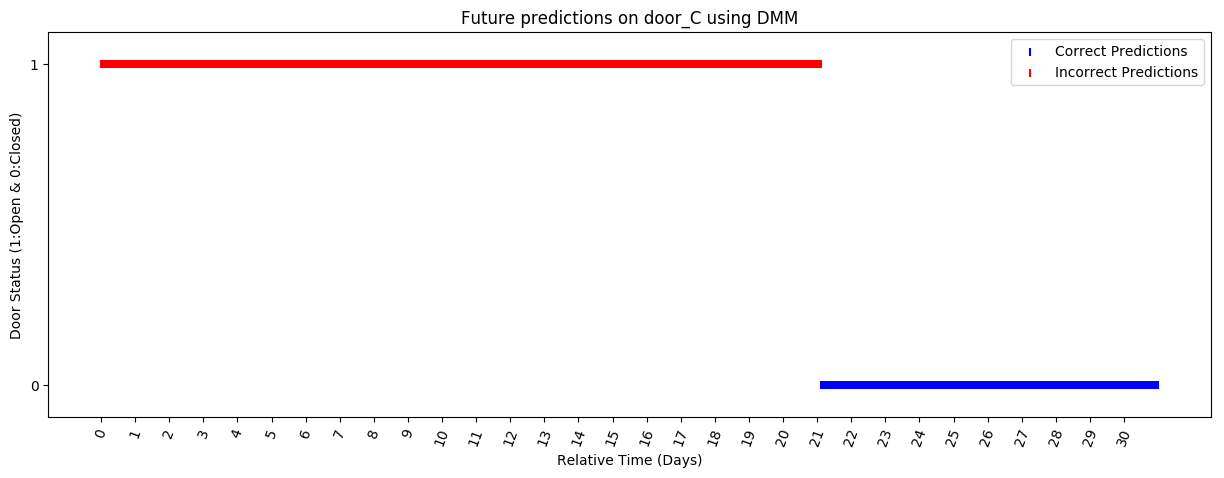
\includegraphics[width = 6in]{images/results/Future_door_C_DMM.png}} \\
    {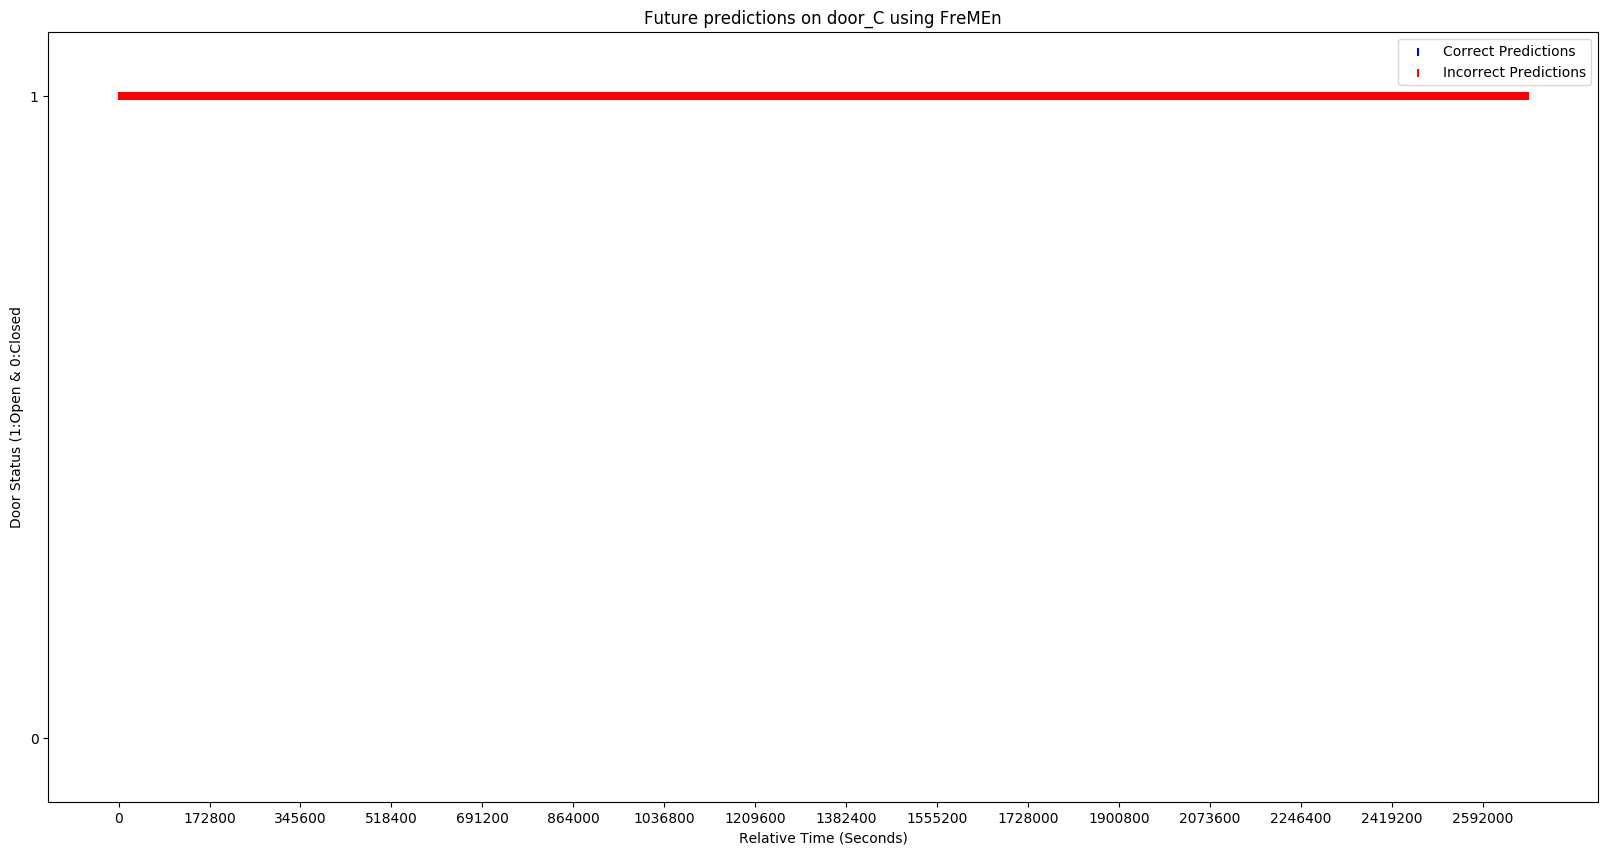
\includegraphics[width = 6in]{images/results/Future_door_C_FreMEn.png}} \\
    {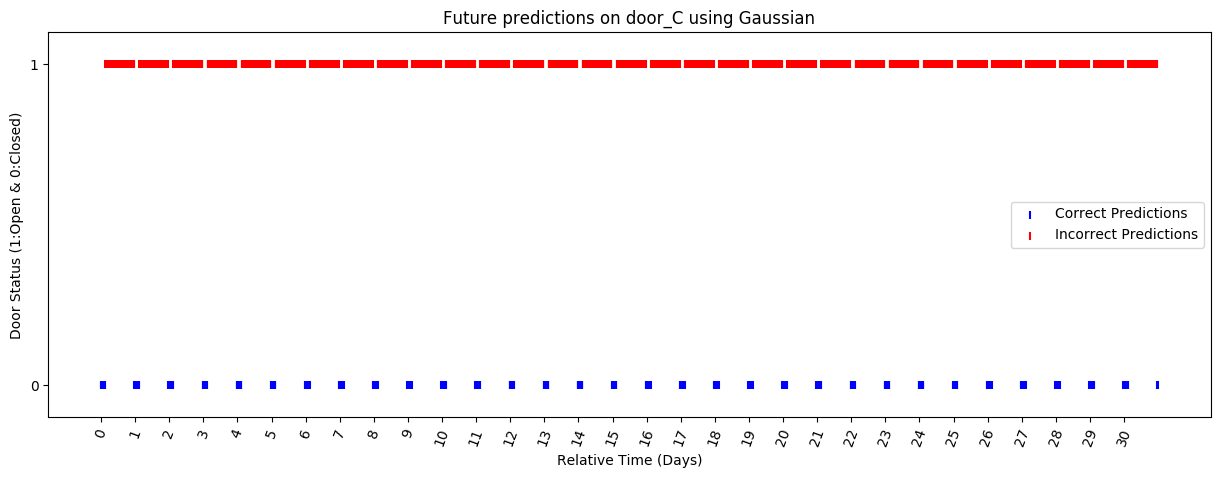
\includegraphics[width = 6in]{images/results/Future_door_C_Gaussian.png}} \\
    {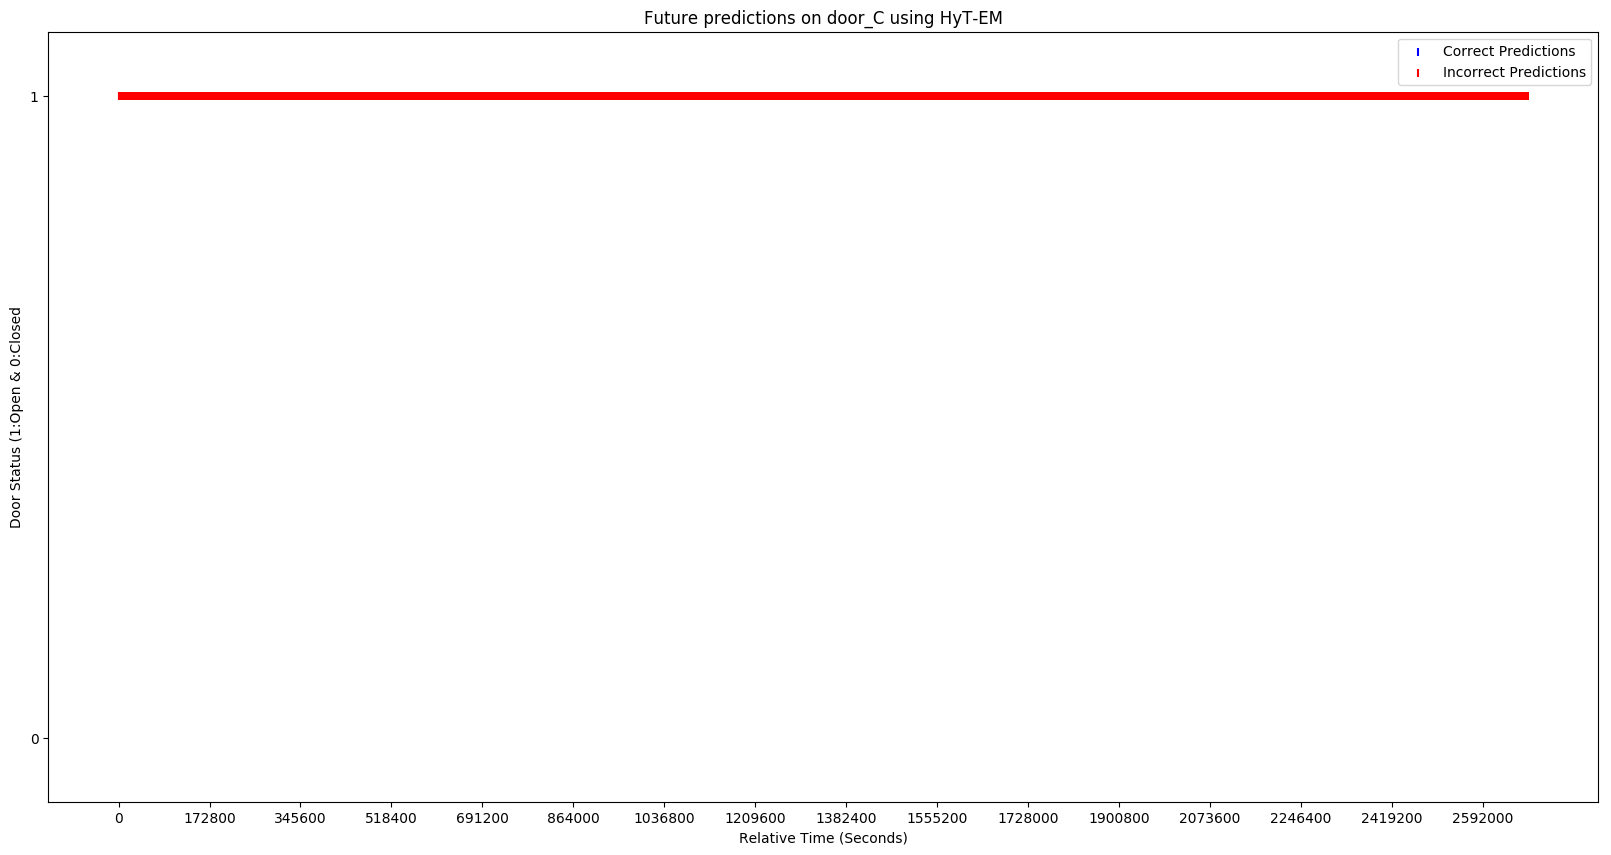
\includegraphics[width = 6in]{images/results/Future_door_C_HyT-EM.png}} \\
  \end{tabular}
  \caption{Future Predictions - Door C}
  \label{figure:future_door_C}
\end{figure}\\ \\

\begin{figure}[!Hp]
  \begin{tabular}{cc}
    {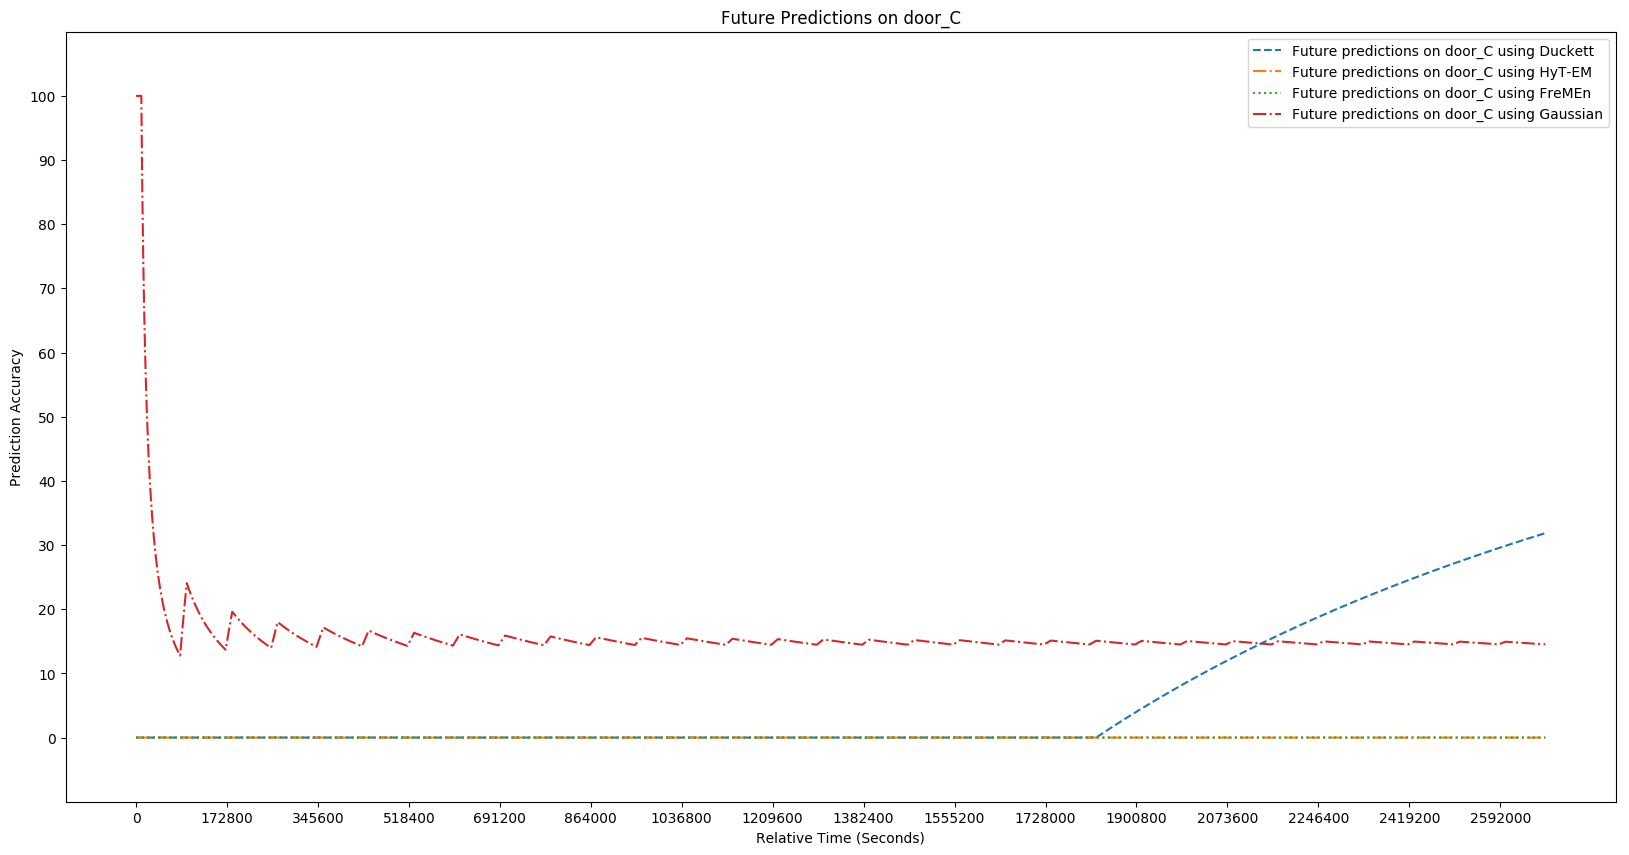
\includegraphics[width = 6in]{images/results/Future_Predictions_on_door_C.png}} \\
    {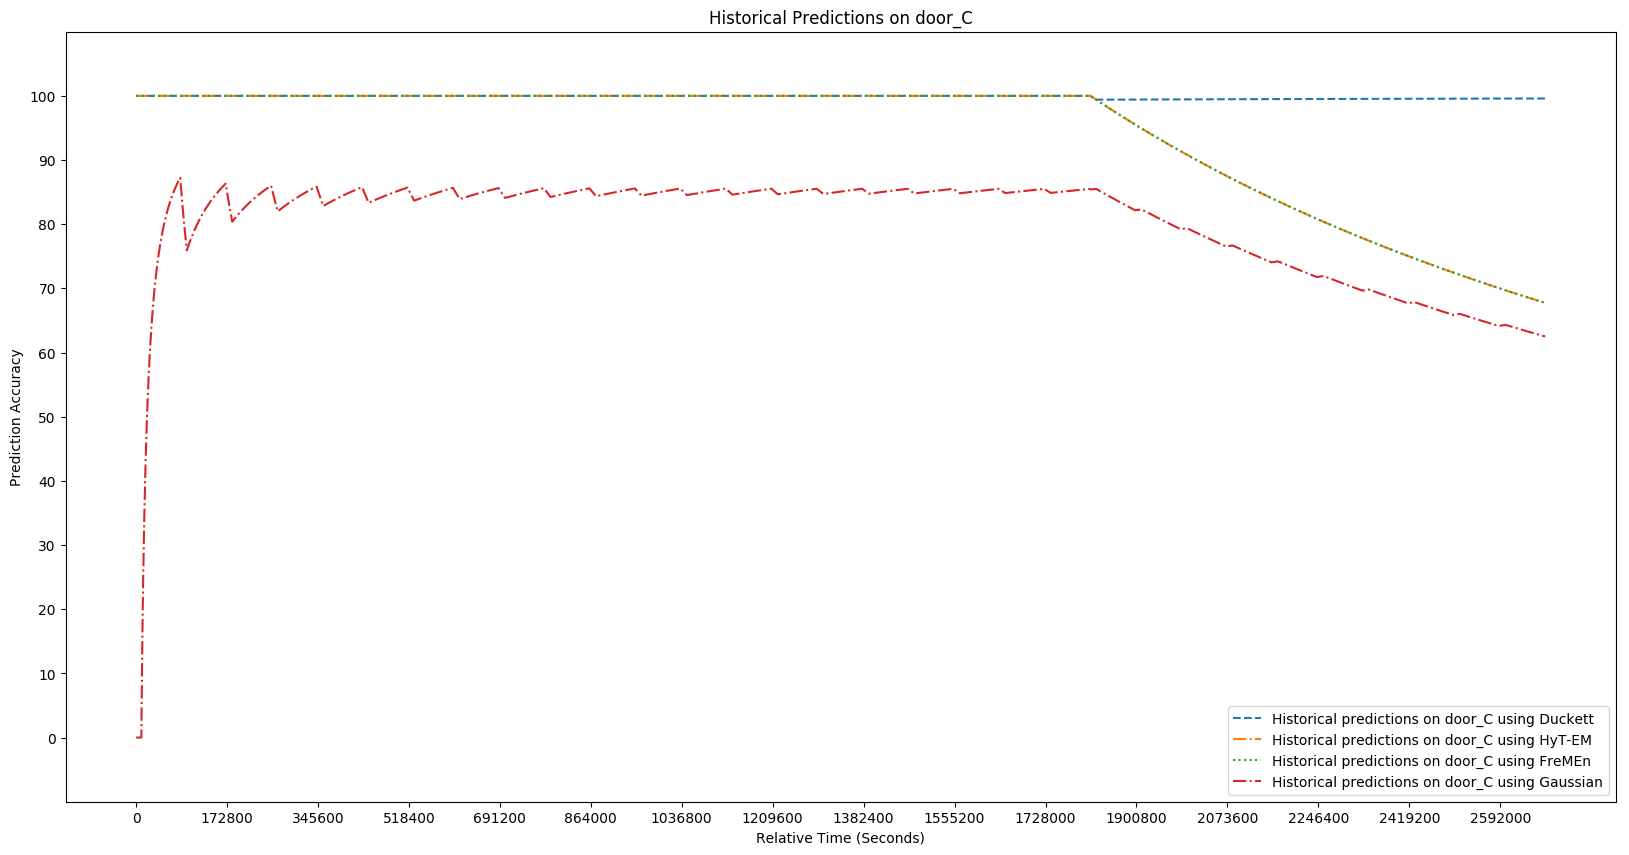
\includegraphics[width = 6in]{images/results/Historical_Predictions_on_door_C.png}} \\
  \end{tabular}
  \caption{Model Accuracy Over Time - Door C}
  \label{figure:accuracy_door_C}
\end{figure}\\ \\
\end{center}


\section{ Congested Hallways }

Having already given an in-depth look at the individual predictions in the
previous section, this section will
focus on metainformation that can be abstracted and
an evaluation of performance with respect to path planning which is the intended primary use case.
To that effect, graphs for every single node are present in the appendix but
have not been included in this section.

\subsection{ Prediction Accuracy Versus Behavior Frequency }

With a moderately large dataset that has varying frequencies such as the one
used for this experiment, it is possible to observe a relationship between the accuracy
of a given spatio-temporal modeling technique and the period of the behavior
attempting to be modeled. In general, the data suggest that behaviors with
a higher frequency are better modeled using Fourier methods like FreMEn and
Hypertime. This is most obvious when looking at behaviors that are repeated multiple
times a day such as the laundry or meal nodes as seen in tables
~\ref{table:Hallway_Laundry_Section},
~\ref{table:Hallway_Meal_Section_0}, and
~\ref{table:Hallway_Meal_Section_1}. In these experiments, the Fourier
methods achieved an impressive 100\% accuracy.
One caveat to these impressive results is the lack of noise
present in the data used for the hallway test. Noise in the data was
explicitly left out of this particular experiment to minimize the variables
present. The presence and effect of noise in data is, however, analyzed in
both the door and elevator experiments. \\

\begin{table}[h!]
  \centering
  \resizebox{\textwidth}{!}{%
    \begin{tabular}{|l|l|l|l|l|}
      \hline
      & DMM & Gaussian & FreMEn  & Hypertime \\ \hline
      Historical Accuracy             & 78.93\% & 26.04\%  & 100.00\% & 100.00\% \\ \hline
      Prediction Accuracy             & 78.93\% & 26.04\%  & 100.00\% & 100.00\% \\ \hline
      Computation Time (Milliseconds) & 610     & 60       & 70       & 1860     \\ \hline
      Memory Usage (KB)               & 30984   & 35160    & 35172    & 37632    \\ \hline
    \end{tabular}%
  }
  \caption{Hallway Laundry Section}
  \label{table:Hallway_Laundry_Section}
\end{table}

\begin{table}[h!]
  \centering
  \resizebox{\textwidth}{!}{%
    \begin{tabular}{|l|l|l|l|l|}
      \hline
      & DMM & Gaussian & FreMEn  & Hypertime \\ \hline
      Historical Accuracy             & 61.63\% & 52.08\%  & 100.00\% & 100.00\% \\ \hline
      Prediction Accuracy             & 61.63\% & 52.08\%  & 100.00\% & 100.00\% \\ \hline
      Computation Time (Milliseconds) & 620     & 60       & 70       & 880      \\ \hline
      Memory Usage (KB)               & 30896   & 35524    & 35600    & 38288    \\ \hline
    \end{tabular}%
  }
  \caption{Hallway Meal Section 0}
  \label{table:Hallway_Meal_Section_0}
\end{table}

\begin{table}[h!]
  \centering
  \resizebox{\textwidth}{!}{%
    \begin{tabular}{|l|l|l|l|l|}
      \hline
      & DMM & Gaussian & FreMEn  & Hypertime \\ \hline
      Historical Accuracy             & 74.93\% & 65.62\%  & 100.00\% & 100.00\% \\ \hline
      Prediction Accuracy             & 74.93\% & 65.62\%  & 100.00\% & 100.00\% \\ \hline
      Computation Time (Milliseconds) & 600     & 60       & 70       & 990      \\ \hline
      Memory Usage (KB)               & 31384   & 35388    & 35588    & 37608    \\ \hline
    \end{tabular}%
  }
  \caption{Hallway Meal Section 1}
  \label{table:Hallway_Meal_Section_1}
\end{table}


When observing the behavior that occurs with the least frequency, the trash
nodes, table~\ref{table:Hallway_Trash_Section_0} and~\ref{table:Hallway_Trash_Section_0},
the opposite trend is observed. Fourier methods no longer are able to
accurately predict behaviors and their predictions drop to around 66\% accuracy.
This is not believed to be a problem with predicting or modeling behaviors with a
lower frequency, but rather a consequence of the ratio between frequency and
length of observation. It is postulated that
with a larger dataset, achieved by increasing the time of observation while
maintaining the density of observations, the predictions would improve. \\

While Fourier methods appear directly correlated with frequency, DMM
appears to have an inverse relationship with frequency. In the meal and
laundry nodes DMM has a prediction accuracy between around 60\% to 80\%.
Furthermore, the lowest prediction accuracy, 61.63\% is found on the meal
node that happens to have the highest number of changes per day. It is likely
that the poor behavior of DMM on behaviors with high frequency is due to
how the averages are stored and computed. DMM undergoes a type of
thrashing wherein by the time the model has adjusted to the current state of a given
behavior the behavior has already changed and the model is again incorrect. It is important to note, that if prior knowledge
or a previous dataset is known, the model parameters such as refresh rate
can be tuned to best fit the frequency of a given behavior.
However, this would have to be done for every behavior, or at least a set or class
of given behaviors and a method to accomplish this on a large scale or automatically does not exist. Finally, in regard to performance in
respect to frequency
DMM fails to accurately predict behaviors that have periods that do not
fall on month boundaries. This is behavior is similar to what happened in the door B experiment.
Additionally, there is a visible difference between historical
and future prediction accuracy for the trash sections, which drop from
91.13\% to 32.13\% in the trash 0 node. Once again, this is not a direct failure
of the DMM model itself, but a result of forcing DMM to make long
term predictions. Its historical predictions are much more accurate to its
real-world behavior as DMM is more like
an online learning model, changing it's predictions after every few observations,
than an offline learning model that trains on a set of data. \\




\begin{table}[htb!]
  \centering
  \resizebox{\textwidth}{!}{%
    \begin{tabular}{|l|l|l|l|l|}
      \hline
      & DMM & Gaussian & FreMEn  & Hypertime \\ \hline
      Historical Accuracy             & 92.31\% & 55.24\%  & 96.17\% & 99.83\%   \\ \hline
      Prediction Accuracy             & 68.92\% & 55.24\%  & 95.97\% & 99.87\%   \\ \hline
      Computation Time (Milliseconds) & 610     & 60       & 90      & 6790      \\ \hline
      Memory Usage (KB)               & 31032   & 35660    & 35520   & 38372     \\ \hline
    \end{tabular}%
  }
  \caption{Hallway Delivery Section}
  \label{table:Hallway_Delivery_Section}
\end{table}

\begin{table}[htb!]
  \centering
  \resizebox{\textwidth}{!}{%
    \begin{tabular}{|l|l|l|l|l|}
      \hline
      & DMM & Gaussian & FreMEn  & Hypertime \\ \hline
      Historical Accuracy             & 91.13\% & 61.49\%  & 64.52\% & 64.52\%   \\ \hline
      Prediction Accuracy             & 32.26\% & 64.05\%  & 63.21\% & 67.74\%   \\ \hline
      Computation Time (Milliseconds) & 600     & 60       & 70      & 1140      \\ \hline
      Memory Usage (KB)               & 31120   & 35364    & 35552   & 37192     \\ \hline
    \end{tabular}%
  }
  \caption{Hallway Trash Section 0}
  \label{table:Hallway_Trash_Section_0}
\end{table}

\begin{table}[htb!]
  \centering
  \resizebox{\textwidth}{!}{%
    \begin{tabular}{|l|l|l|l|l|}
      \hline
      & DMM & Gaussian & FreMEn  & Hypertime \\ \hline
      Historical Accuracy             & 90.96\% & 61.09\%  & 67.74\%  & 67.74\% \\ \hline
      Prediction Accuracy             & 35.79\% & 61.09\%  & 67.74\%  & 67.74\% \\ \hline
      Computation Time (Milliseconds) & 610     & 60       & 70       & 2120    \\ \hline
      Memory Usage (KB)               & 31116   & 35400    & 34928    & 37520   \\ \hline
    \end{tabular}%
  }
  \caption{Hallway Trash Section 1}
  \label{table:Hallway_Trash_Section_1}
\end{table}


\subsection{ Terminology and Metrics }

In order to accurately and fairly compare the path planning results, terminology
was devised to describe the mistakes made when planning with the use of a models
predictions. Errors encountered when attempting to execute a path produced
using a models predictions were grouped into two categories: hard errors \&
soft errors. \\

Hard errors are errors that cause issues that are impossible for
a robot to theoretically recover from. This only happens when the ground truth
path and the model predicted plan are at odds. That is to say, hard errors are
when the ground truth claims a path is not currently possible and the predicted
model claims there exists a valid path or vice versa. \\

Soft errors are errors that occur when the ground truth path and the model
predicted path both agree on the existence of a path, but disagree on the
specifics. This means that soft errors only occur when there exists a path
to the goal, but the model predicted path is either too long or would cause
the robot to run into an area with obstacles. However,
by evaluating the ground truth it can be known that a path is possible and thus the robot in theory could
create another plan with this newly discovered information. This newly planned path would then allow
the robot to reach it's goal. \\

Assuming that the path produced by the model is valid, the path
length is calculated and then compared against the ground truth path. Since
both hard and soft errors produce invalid paths, they are not used to
calculate the number of average cells traveled. This number is used as a quick and
easy way of calculating the efficiency of paths generated when using a given
spatio-temporal world model. \\

As mentioned in the previous section, there is no noise introduced
into the simulated data. Thus, aside from DMM, the historical and future
predictions are, for all intents and purposes identical. The reasons for this
will be discussed in the section below, but because of this, only the future
path planning results will be analyzed. \\

Finally, it is important to note that although all of the behaviors were
combined to produce a path prediction the models were not simultaneously
trained and asked to predict the various behaviors. Instead, each behavior,
similar to the door experiment, was predicted individually and sequentially.
Therefore, in order to have an overview of the resources used, the total
time spent on planning was calculated by summing up each of the individual
times it took to train a specific model. Due to the fact that this was happening
sequentially, not simultaneously, memory usage can then be taken as an
average or a maximum over time. A maximum was chosen as it is assumed that
memory is a finite resource that does not change over time and therefore as long
as a system has the minimum amount of memory available to meet a programs'
maximum demands there will not be any issues during run-time.
In the future, if this was turned into a multi-threaded process the sum may wished to be used.
A naive and safe assumption if this figure is desired otherwise is to simply
multiply the maximum amount of memory used by the number of objects for which
a predictive model is desired. \\

\begin{table}[htb!]
  \centering
  \resizebox{\textwidth}{!}{%
    \begin{tabular}{|l|l|l|l|l|}
      \hline
      & DMM & Gaussian & FreMEn  & Hypertime \\ \hline
      Percent Hard Errors                & 60.15\% & 81.25\% & 50.00\% & 50.00\% \\ \hline
      Percent Soft Errors                & 14.92\% & 2.08\%  & 2.69\%  & 2.69\%  \\ \hline
      Average Additional Cells Traversed & 5.74    & 6.34    & 3.12    & 3.12    \\ \hline
      Total Time Spent Planning          & 3650    & 360     & 440     & 13780   \\ \hline
      Maximum Memory Usage               & 31384   & 35660   & 35588   & 38372   \\ \hline
    \end{tabular}%
  }
  \caption{Future Path Planning Results}
  \label{table:Future_Path_Planning_Results}
\end{table}




\subsection{ Path Planning Results }

Figure \ref{fig:G_FP_res} shows the various models' performance metrics over
simulated time. It is the goal of the models to reduce the number of errors
and additional distance traveled when providing information for path planning.
Thus the methods with the lowest lines on the graph are the most
preferable methods. Using this general rule, it is clear that the Fourier
methods have achieved the best results with a tie for both hard and soft errors
amongst themselves. They are beaten out by Gaussian Mixture Models for soft
errors, but this is only due to the significant number of hard errors that
the Gaussian Mixture Model achieved. With so many hard errors, the method
didn't have the opportunity to commit as many soft errors. Additionally,
because hard errors imply the complete failure to predict if the goal is
achievable they are substantially worse. \\

One notable effect of using each of the multiple behavior predictions to do path
planning is that there is an averaging effect over the data. Individual mistakes
or incorrect predictions don't always make or break a plan. One place this is
extremely obvious is in DMM's prediction of high frequency events.
Despite the disparity between historical and future predictions for DMM in
terms of these individual behavior prediction, the only difference in the final
metrics are two additional soft errors during future predictions. This may be
because of the large number of hard errors encountered preventing more
soft errors from being generated, similar to the Gaussian Mixture Model.
Another factor for this smoothing behavior is the location of the
various behaviors and how they relate to a plan being possible. \\

In terms of computational cost, the path planning results appear to roughly
scale linearly with the previous individual experiments results with minor
deviations. The maximum memory used hovers between 30 to 40 megabytes for all
of the experiments much like before. Similarly, DMM takes an order of
magnitude longer than Gaussian Mixture Models and FreMEn to produce results.
Hypertime again takes another order of magnitude longer than DMM taking
almost 14 seconds However, a large disparity is visible when looking at the
sum of time taken to produce a path. Despite taking less than 30 times as long
to produce results, FreMEn achieved the same prediction and path planning
performance as Hypertime.


\begin{center}
  \begin{figure}[!Hp]
  \begin{tabular}{cc}
    {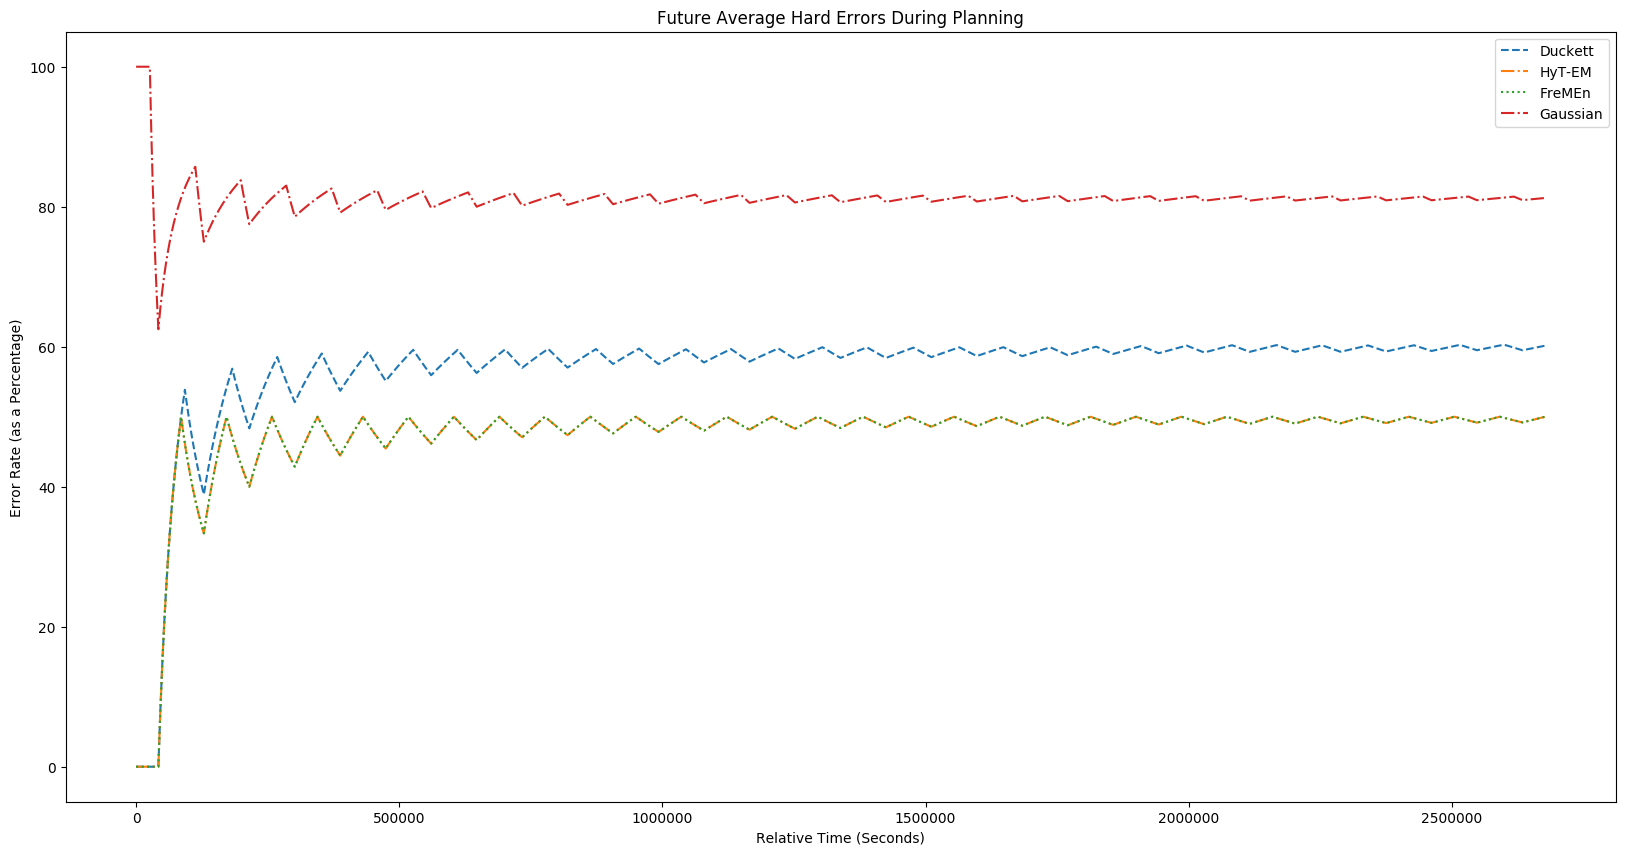
\includegraphics[width = 6in]{images/results/Future_Average_Hard_Errors_During_Planning.png}} \\
    {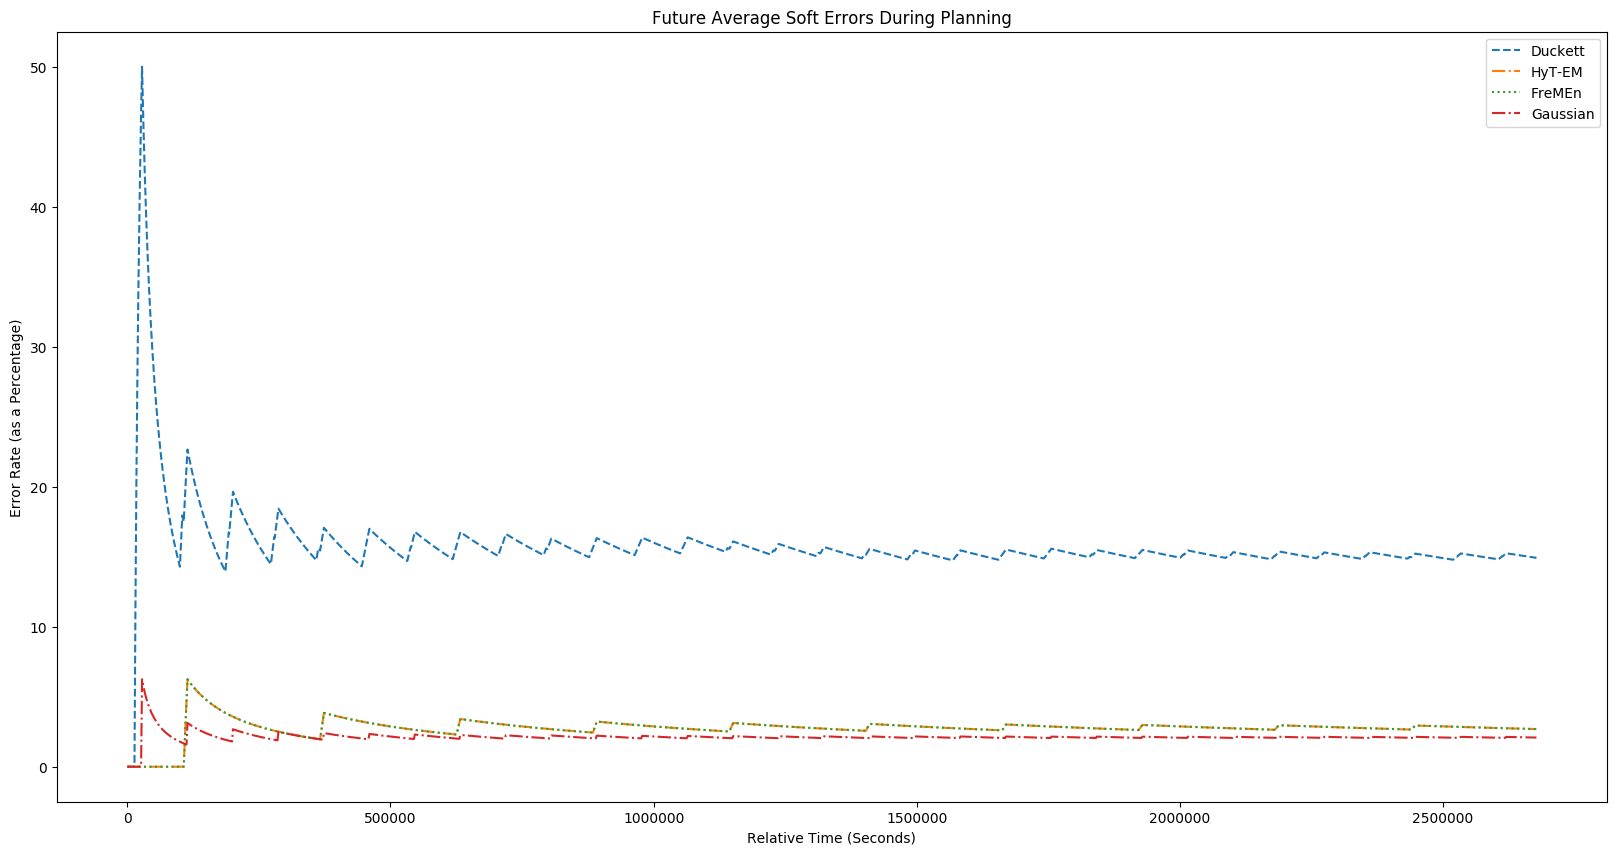
\includegraphics[width = 6in]{images/results/Future_Average_Soft_Errors_During_Planning.png}} \\
    {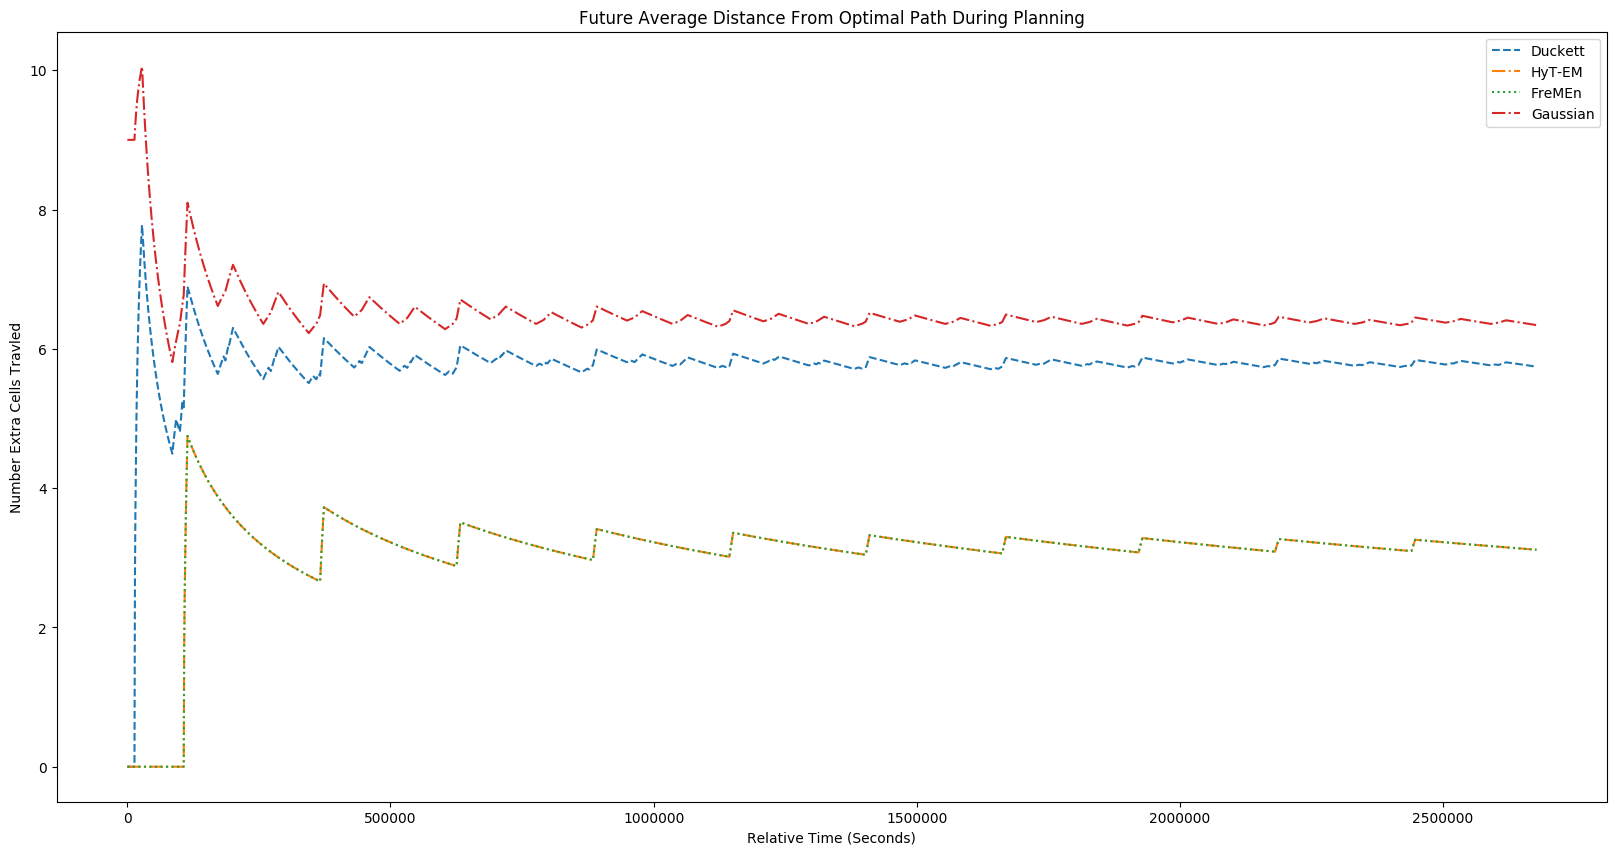
\includegraphics[width = 6in]{images/results/Future_Average_Distance_From_Optimal_Path_During_Planning.png}} \\
  \end{tabular}
  \caption{ Future Planning Results}
  \label{fig:G_FP_res}
\end{figure}
\end{center}



\section{ Busy Elevators }

\subsection{ Classification Methods }

Upon even a cursory glance at the resulting graphs, such as the one in figure
~\ref{figure:Future_Predictions_Elevator_Data}, it is immediately
obvious that each model has a different approach to classification and
prediction of the data. DMM, which predicts by
averaging each of its sub-models, is perhaps the easiest to understand at first
glance. It results in a somewhat smooth curve that follows the training data
extremely closely. \\

On the other hand, Gaussian Mixture Models and FreMEn take a drastically
different approach. Since, at their core they are binary classifiers, the
prediction methods' as described in Section 5 result into two distinct
prediction options. Both method's predictions hover around 0 and 7, although
not exactly on an integer boundary. It is clear the lower value is close to 0
due to the large amount of time the elevator spends at what is essentially a
rest state with next to no use. This is mostly between the hours of 22:00 and
08:30 or 10.5 hours. The other prediction that hovers around 7
is slightly harder to predict with precision but can be roughly estimated when
looking at the nominal times for waiting. When ruling out values that would be
placed into a 0 prediction, there are a large amount of nominal values between 4
and 9 which average out to 6.5. Finally, due to the large amount of noise
combined with the fact that an elevator cannot have a negative wait time,
the average is pulled up a bit by the extremely long wait times that can be
as high as 30 seconds during peak hours. \\

\begin{center}
  \begin{figure}[!Hp]
  \begin{tabular}{cc}
    {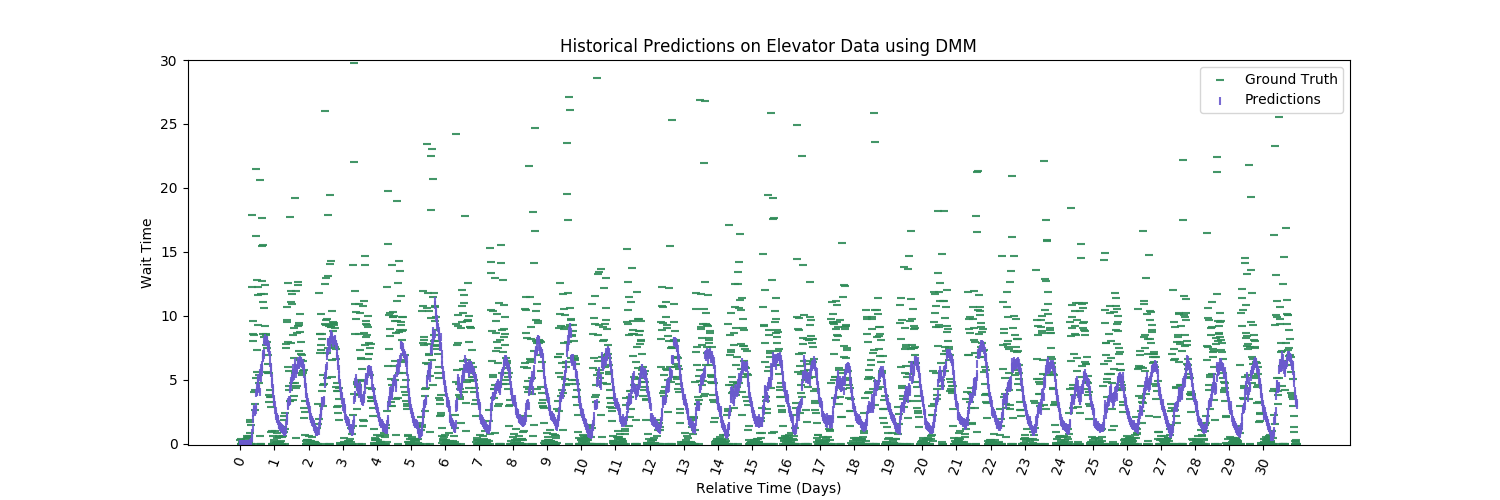
\includegraphics[width = 6in]{images/results/Historical_elevator_DMM.png}} \\
    {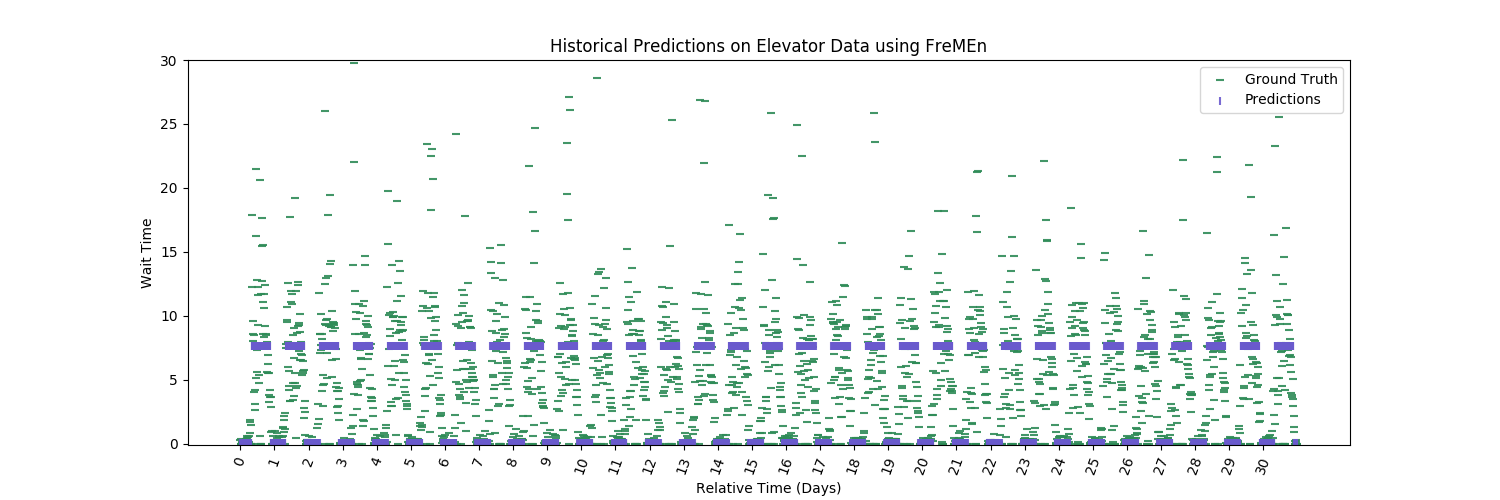
\includegraphics[width = 6in]{images/results/Historical_elevator_FreMEn.png}} \\
    {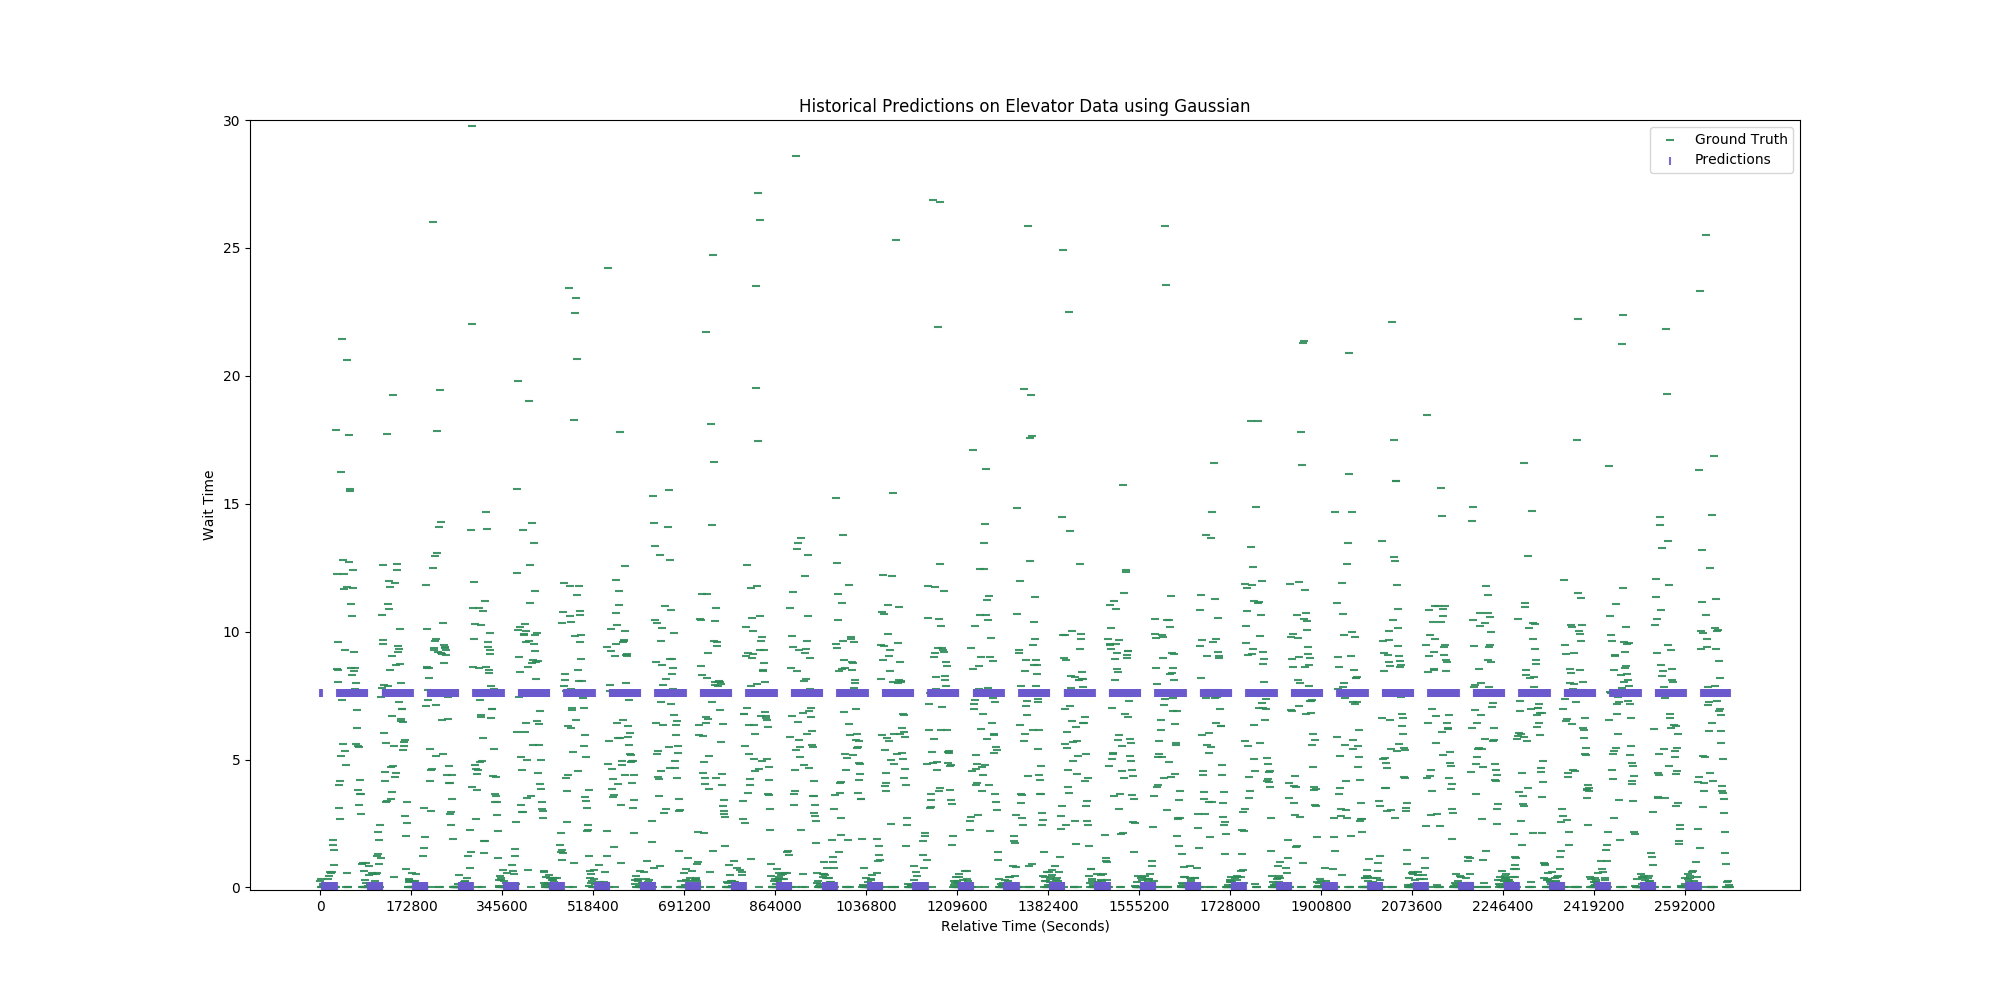
\includegraphics[width = 6in]{images/results/Historical_elevator_Gaussian.png}} \\
    {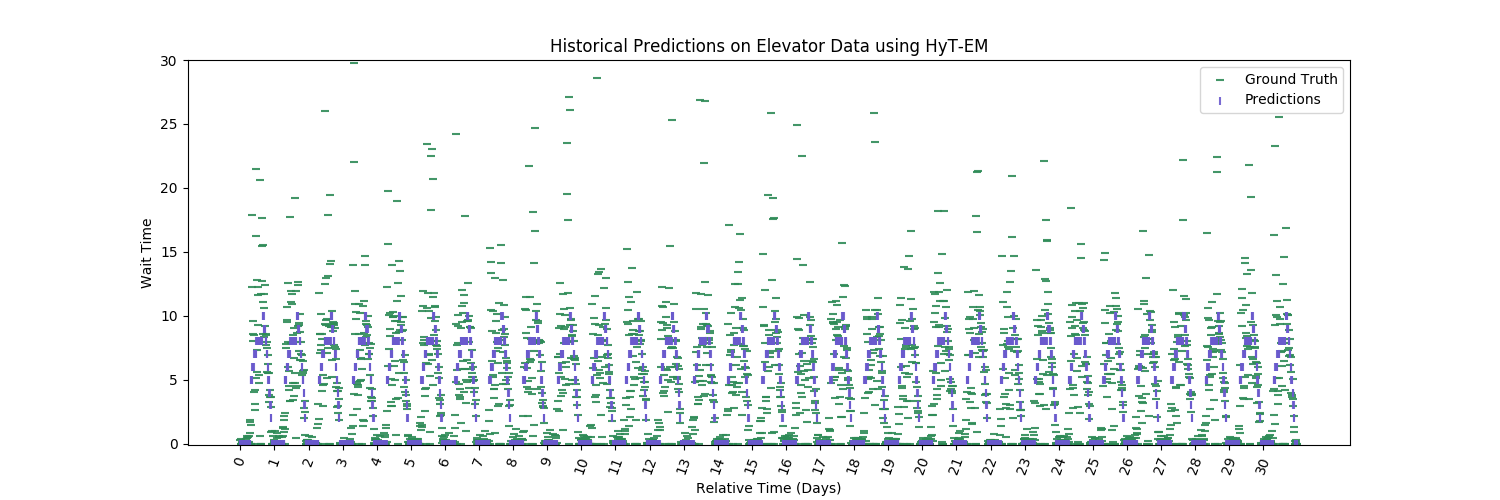
\includegraphics[width = 6in]{images/results/Historical_elevator_HyT-EM.png}} \\
  \end{tabular}
  \caption{Historical Recreations - Elevator Data}
  \label{figure:Historical_Recreations_Elevator_Data}
\end{figure}

\begin{figure}[!Hp]
  \begin{tabular}{cc}
    {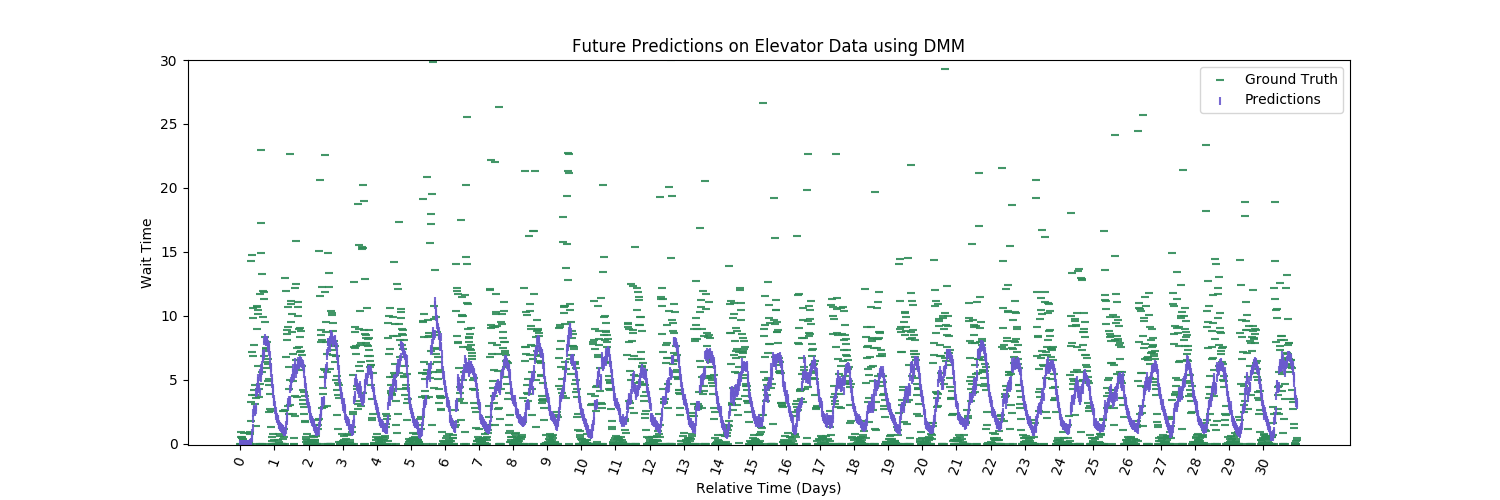
\includegraphics[width = 6in]{images/results/Future_elevator_DMM.png}} \\
    {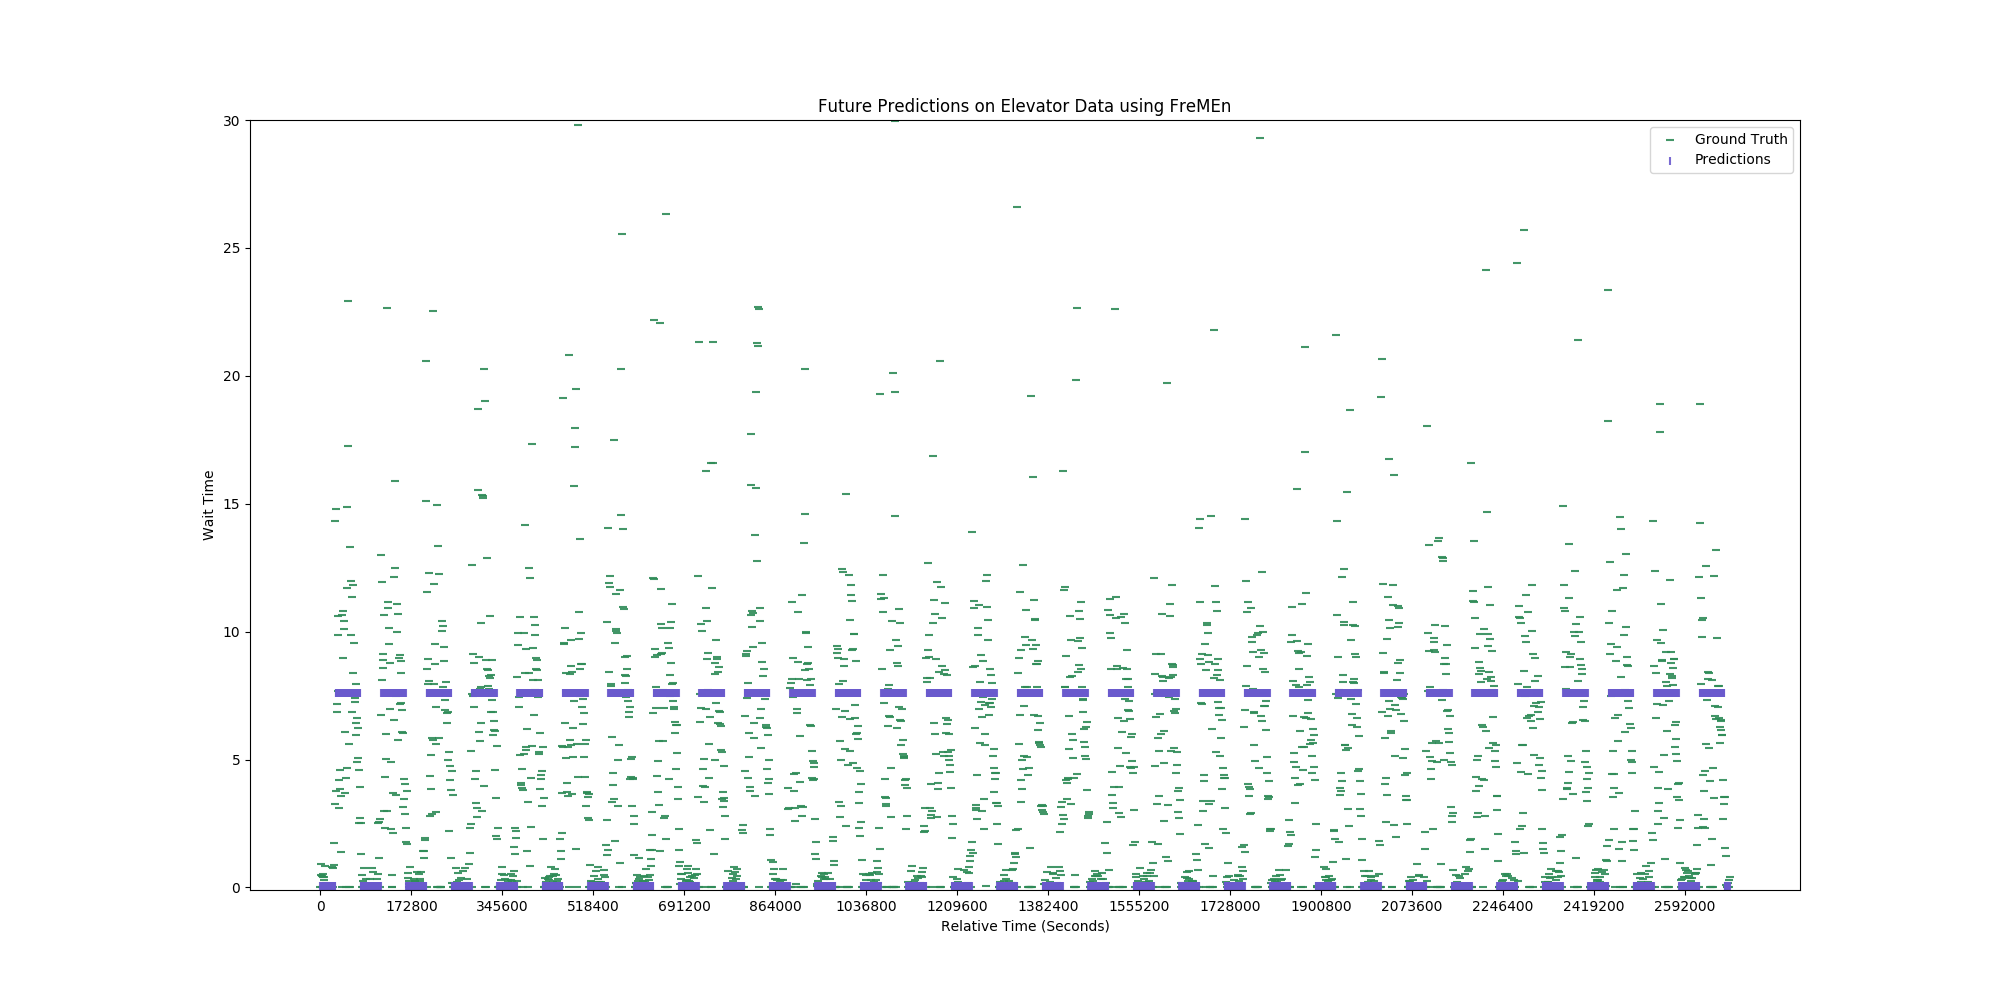
\includegraphics[width = 6in]{images/results/Future_elevator_FreMEn.png}} \\
    {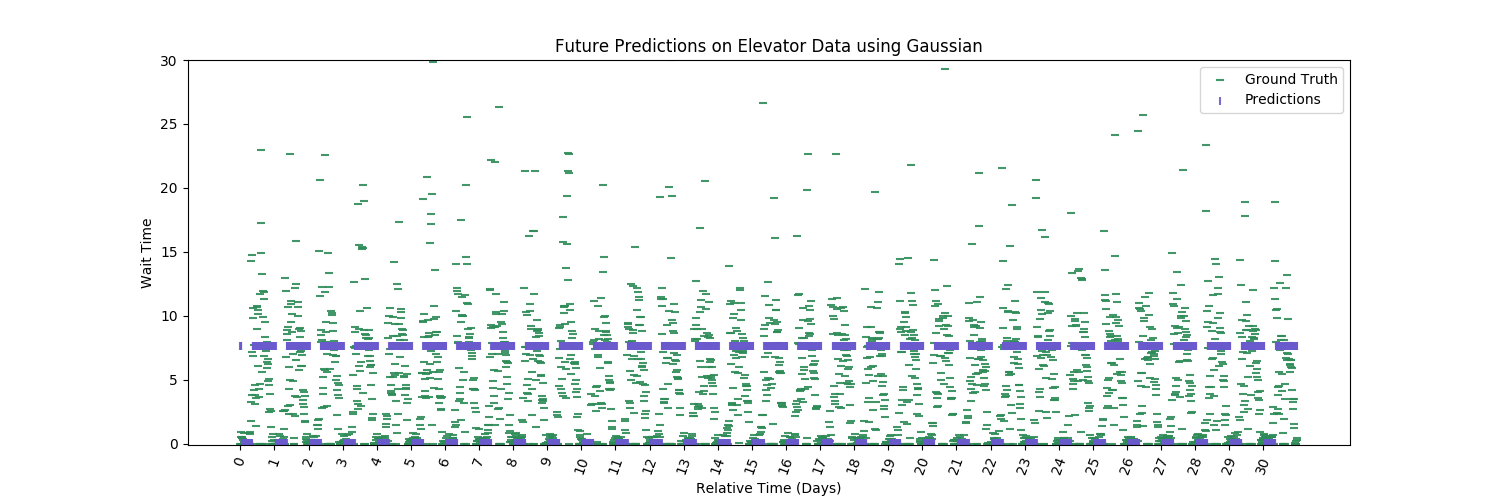
\includegraphics[width = 6in]{images/results/Future_elevator_Gaussian.png}} \\
    {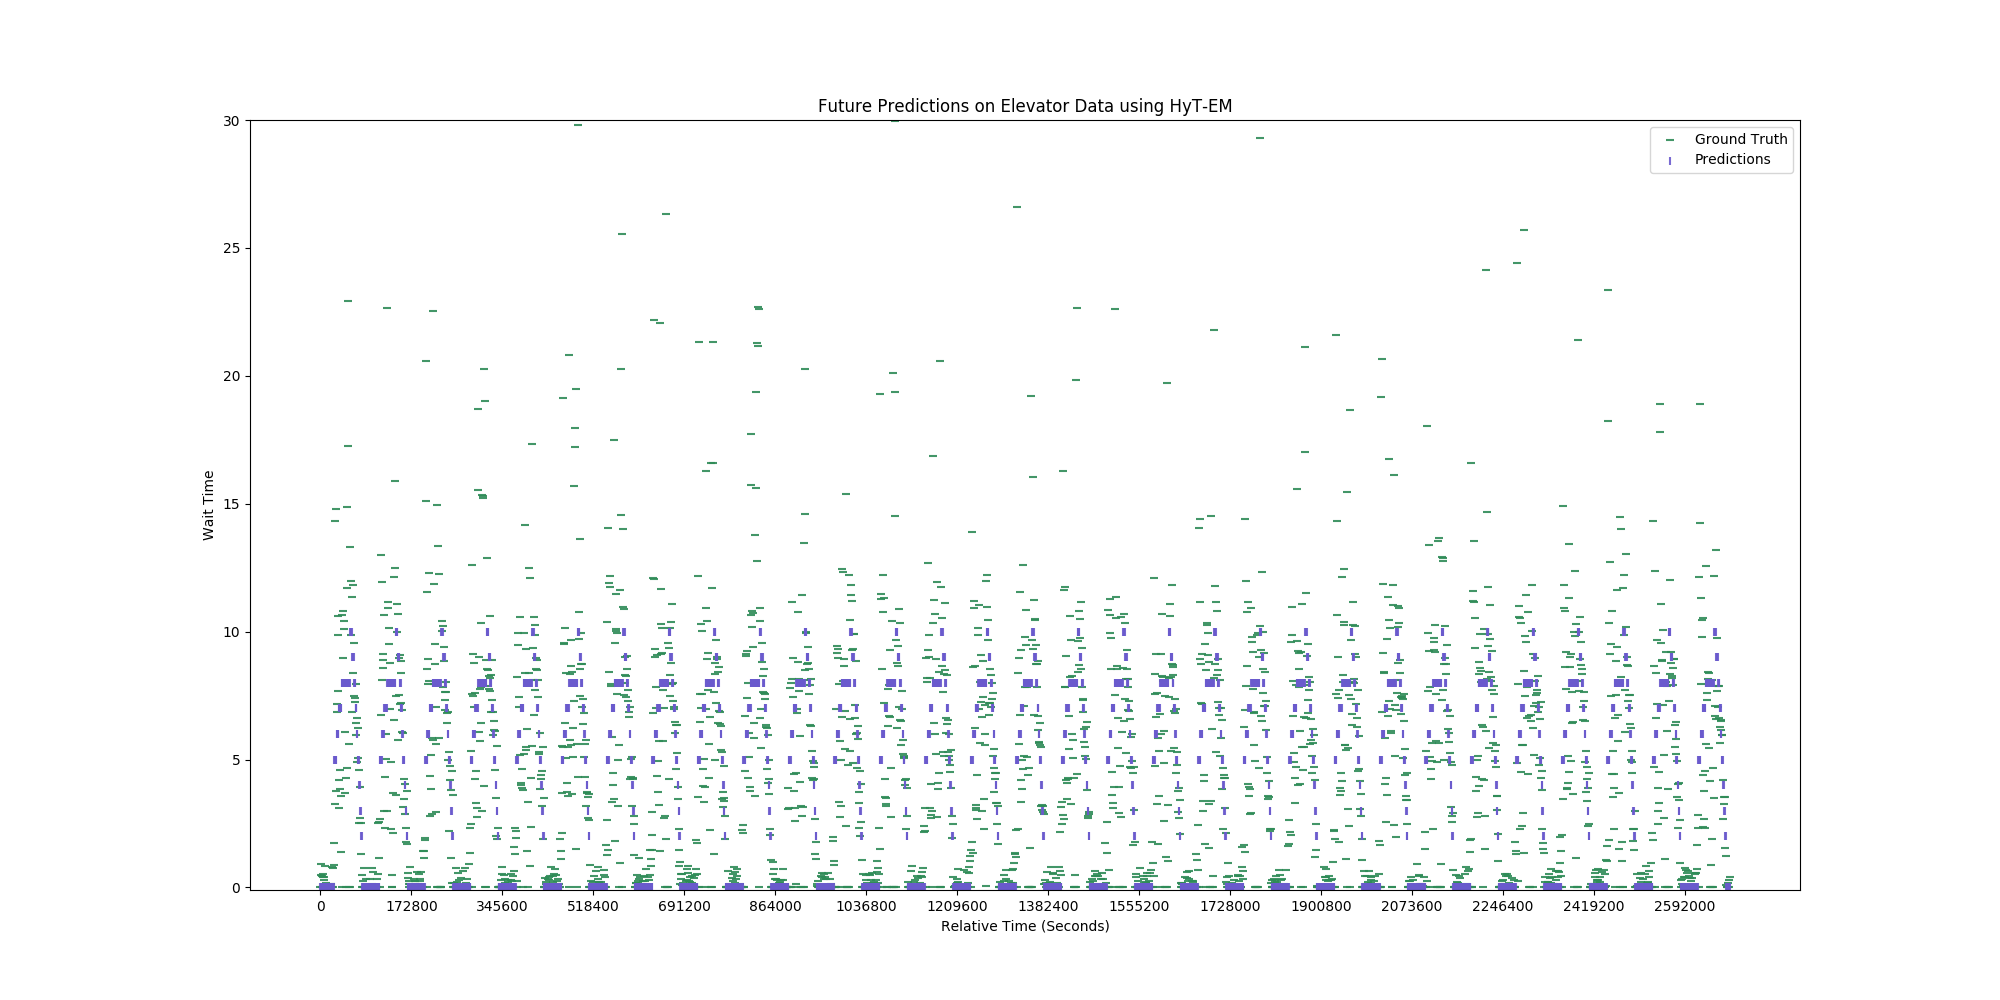
\includegraphics[width = 6in]{images/results/Future_elevator_HyT-EM.png}} \\
  \end{tabular}
  \caption{Future Predictions - Elevator Data}
  \label{figure:Future_Predictions_Elevator_Data}
\end{figure}
\end{center}


Finally, and perhaps most interesting, are the Hypertime results. Hypertime takes a
unique approach to classifying its data. Once again, looking at the Hypertime
graph in figures~\ref{figure:Historical_Recreations_Elevator_Data} and
~\ref{figure:Future_Predictions_Elevator_Data}
it is seen that predictions are clustered on integer boundaries. To be clear,
non-binary Hypertime in its current implementation, although capable of training
on real data\footnote[1]{Real data as in both real-world data and all the numbers in the set of real numbers that can be represented using standard floating point notation},
can only produce
integer predictions. This limitation is due to how predictions are evaluated
before being accepted as the actual prediction for a given time.
When producing a prediction, or an
estimate as referred to in Hypertime, ``the likelihood distribution of the
sample having a given value at time t''
\footnote[2]{This is a comment taken from the Hypertime source code. Particularly the estimate function in CHyperTime.cpp}
is calculated
for each sample from 0 until a maximum value. A maximum value for 30 was used
for this experiment. This means that during calculation Hypertime would never
be able to predict a wait time of 30 seconds or greater. Looking again at the
resulting figures, it is clear this is not an issue as there does not appear to
be any prediction greater than 10 seconds. Thus, with no predictions even
nearing 30, it is reasonable to conclude that the upper limit did not hamper the ability for
the model to produce accurate predictions. \\

\subsection{ Metrics }

The only additional metric included in this experiment was that of ``Average
Distance from Correct Wait Time''. This, as the name implies, simply takes the
difference between a models predicted wait time and the ground truth wait time
provided in the data. The absolute value of this difference is saved and then
averaged for every time step to illustrate how the average changes over time. This
metric does not make a differentiation between the robot waiting for the
elevator versus the elevator waiting for the robot. No other additional
factors have been taken into account. Specifically, this includes something like calling an
elevator so far in advance that the elevator shows up and is called by someone else. \\

\subsection{ Performance \& Scalability }

\begin{table}[h!]
  \centering
  \resizebox{\textwidth}{!}{%
    \begin{tabular}{|l|l|l|l|l|}
      \hline
      & DMM & Gaussian & FreMEn  & Hypertime \\ \hline
      Historical Average Additional Wait Time (Seconds)     & 3.05    & 3.24     & 2.13    & 1.90      \\ \hline
      Future Average Additional Wait Time (Seconds)         & 3.06    & 3.25     & 2.12    & 1.92      \\ \hline
      Computation Time (Milliseconds)                       & 610     & 60       & 70      & 7690      \\ \hline
      Memory Usage (KB)                                     & 31092   & 34636    & 34672   & 67788     \\ \hline
    \end{tabular}%
  }
  \caption{Elevator Wait Time Overview}
  \label{table:Elevator_Wait_Time_Overview}
\end{table}


\begin{table}[h!]
  \centering
  \resizebox{\textwidth}{!}{%
    \begin{tabular}{|l|l|l|l|l|}
      \hline
      & DMM & Gaussian & FreMEn  & Hypertime \\ \hline
      Historical Average Additional Wait Time (Seconds)     & 1.58    & 4.47     & 2.05    & 1.58      \\ \hline
      Future Average Additional Wait Time (Seconds)         & 1.65    & 4.47     & 2.05    & 1.59      \\ \hline
      Computation Time (Milliseconds)                       & 7350    & 90       & 350     & 250037    \\ \hline
      Memory Usage (KB)                                     & 75304   & 35140    & 34980   & 79864     \\ \hline
    \end{tabular}%
  }
  \caption{High Resolution Elevator Wait Time Overview}
  \label{table:High_Resolution_Elevator_Wait_Time_Overview}
\end{table}

Table~\ref{table:Elevator_Wait_Time_Overview} shows similar results to those
in previous sections with a few notable exceptions. Foremost, computation time
remains mostly consistent, with Gaussian Mixture Models and FreMEn coming in at
the upper tens of milliseconds, DMM an order of magnitude higher and
Hypertime being yet another order of magnitude higher than DMM. Hypertime,
although remaining under 10 seconds, does take slightly longer than would
be expected compared to previous results. This extra time is likely to originate
from the switch from binary to non-binary state classification. As mentioned previously,
when doing non-binary classification Hypertime must check every integer value
from 0 until a maximum prediction value, which in this experiment was 30. Had this
number been reduced to something closer to 10 (the maximum experimentally
predicted value) it is likely that the computation time would have been
reduced to 2 or 3 seconds placing it closer to previous experiments but with a
slightly longer time due to the additional calculations needed. This same
trend and effect is mirrored in memory usage for the same reasons. \\

Finally, prediction wise, once again similar results are visible. Hypertime
has the best results with under 2 seconds of average distance from the correct
wait time, FreMEn trailing slightly behind at barely over 2 seconds, DMM and
then Gaussian both over 3 seconds. \\

Overall, the results are not particularly surprising when looking at previous
experiments, until the results in Table
~\ref{table:Elevator_Wait_Time_Overview} are compared with the results in Table
~\ref{table:High_Resolution_Elevator_Wait_Time_Overview}. The High Resolution
data, sampled at a rate of once per minute instead of once per 15 minutes,
highlights and exemplifies the data found in the lower resolution data. \\

Perhaps the most obvious and most interesting change is the drastic improvement
in DMM, which halved its wait time error over the lower resolution data.
The main conclusion to be drawn from this is the importance of tuning DMM
to refresh its internal representation of objects with the expected occurrence
of periodic changes with respect to the rate at which that data is being
sampled. DMM struggles to predict changes in daily behavior when samples
occur at 15 minute increments as seen both in the low resolution data for the
elevator and the meal nodes back in the navigation experiment.
Additionally, a tenth of a second decrease in wait time prediction is now much more obvious.
In the real-world this would not be a significant problem,
but it shows issues with long-term future predictions. \\

Figure~\ref{figure:Model_Accuracy_Over_Time_Elevator_Data} shows an overview
of the different models over time. Slight movement was seen in either direction for Gaussian Mixture Models and
FreMEn. The simplistic nature of the Gaussian Mixture Models results in roughly
a 1 second decrease in prediction accuracy, but it does manage to maintain resource
usage very close to that of the lower density data. This suggests that Gaussian
Mixture Models may be a good fit for very large datasets with simplistic
periodic behavior where precise accuracy is not necessary. FreMEn on the other
hand had a slight increase in prediction accuracy but saw a slight increase in
computation time while maintaining memory usage. This increase in
computational time, specifically when compared to Gaussian Mixture Models,
likely comes from the model order FreMEn operates at (3), which causes
three loops through the training data for predictions. Since the loops are
merely over the same training data, but with different parameters for estimation
it would make sense the computation time would increase while memory usage would
stay relatively constant. In fact, a rough calculation shows just this. Gaussian
Mixture Models take about 30 milliseconds longer in the high resolution data,
an increase from 60 to 90. Adding an additional 30 milliseconds to FreMEn's
low resolution computation time value of 70 yields 100 milliseconds. Accounting
for the additional work done by FreMEn by multiplying by 3 yields around 300
milliseconds. This is close to the observed 350 milliseconds, especially when
additional overhead is considered. \\

\begin{center}
\begin{figure}[!Hp]
  \begin{tabular}{cc}
    {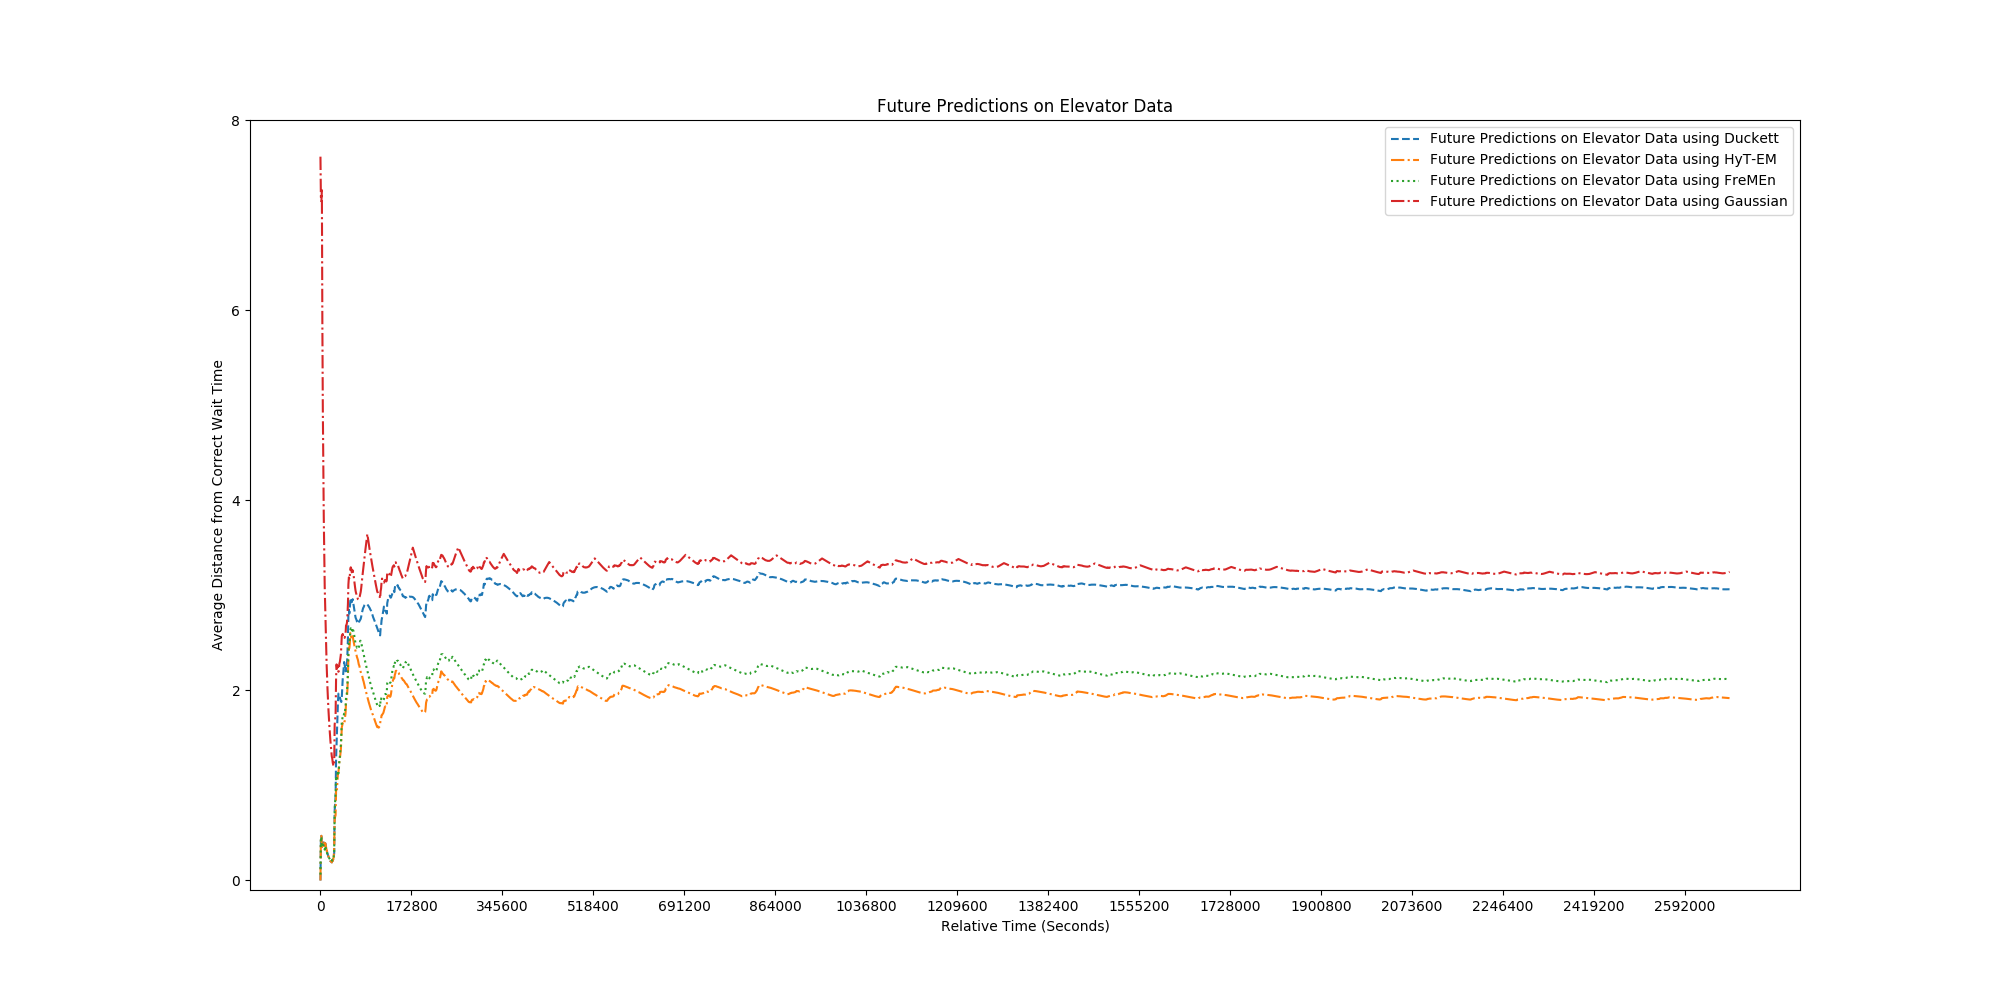
\includegraphics[width = 6in]{images/results/Future_Predictions_on_Elevator_Data.png}} \\
    {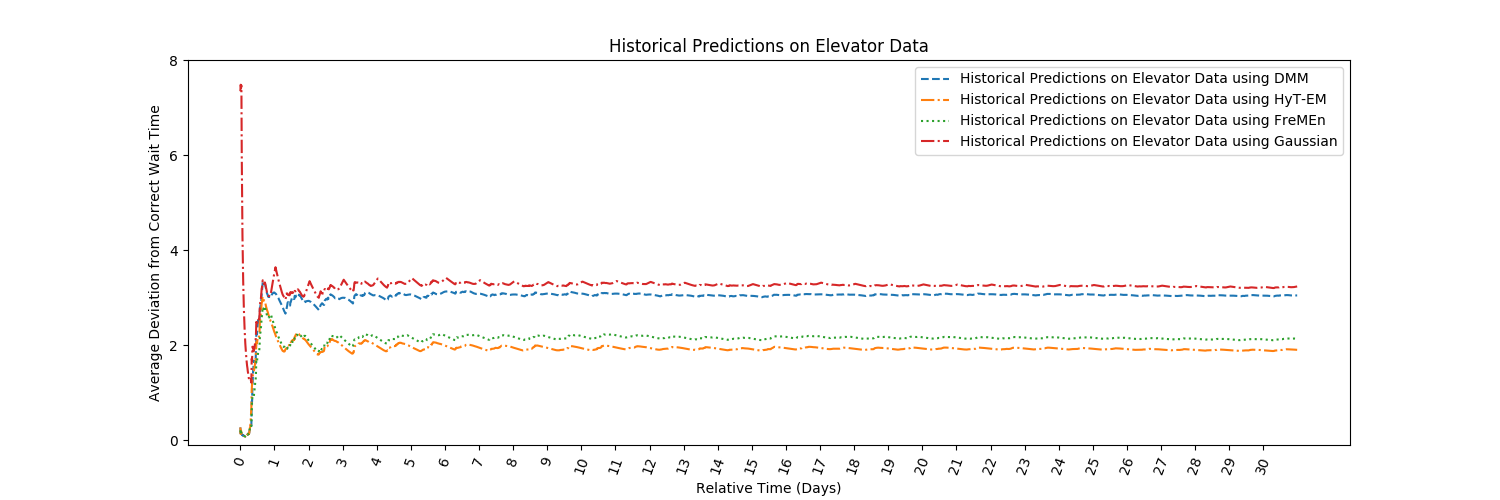
\includegraphics[width = 6in]{images/results/Historical_Predictions_on_Elevator_Data.png}} \\
  \end{tabular}
  \caption{Model Accuracy Over Time - Elevator Data}
  \label{figure:Model_Accuracy_Over_Time_Elevator_Data}
\end{figure}
\end{center}


Finally, Hypertime has arguably the most intriguing change between high and low
resolution elevator data. There was only a relatively small increase in memory usage. The computational time, however, saw an
extremely large increase to over 250000 milliseconds, or over 4 minutes. This
additional run-time only yields a performance increase of between 300 and 400
milliseconds. It may be argued that the relatively small increase of prediction
accuracy may be the result of Hypertime being unable to make more accurate
predictions due to its integer limitation. Without this limitation it could
perhaps continue to increase in accuracy but this would only further increase its
computational time. The computational time is likely to have scaled they way it did because of
the large number of calculations done for each data point during the
estimation portion of prediction. As noted previously, in this specific case
30 complex calculations must be done before a single estimation can be chosen at
a given time t. It is important to recall that a reduction in the maximum
prediction value, would most likely reduce the
computational time considerably, perhaps as much as a third of its original
value if the max estimate was limited to 10. This would likely result in a
computational time between 1 and 2.5 minutes. \\


\section{ Final Thoughts }

After reviewing the 3 experiments and 4 methods several trends can be
identified. Starting with computational efficiency, memory usage appeared
relatively consistent through all experiments and methods. With just under 3000
data points per test month and around 30KB of memory used per run
it appeared that each data point takes slightly more than 10 bytes plus
some overhead. This represents the minimum cost for something like DMM although
other methods use slightly more memory. Specifically, when ranked from highest to lowest memory usage,
the order was Hypertime, FreMEn, Gaussian, and DMM. \\

With respect to computational usage in the time domain, a different pattern is
observed. Ignoring minor fluctuation between experiments, Gaussian and FreMEn
consistently used tens or hundreds of milliseconds on 3000 data points.
DMM used an order of magnitude beyond that, and Hypertime used yet another
order of magnitude more. Although this is the average case it would appear that
scaling is not linear for Hypertime as demonstrated in the high resolution
elevator experiment. Future testing will have to be done to determine the
scaling factor. \\

In terms of accuracy, the various methods each had their own strengths and
weaknesses. The Gaussian method was on average a very efficient
technique and consistently was the least accurate when making predictions. It appears the
Gaussian method was only able to make semi-accurate predictions when presented
with data that was highly regular, contained minimal noise, and had a
relatively high frequency of occurrence with respect to the observed time
frame. Osculations are also visible in a large number of the accuracy graphs,
especially in the earlier sections of the graph. These osculations do not
originate from any of the models behavior but instead are a result of how the
averages were computed. Averages were computed over time such that, at the
beginning, only a few data points existed, and thus a few right or wrong
predictions have a large impact. As more an more data points are added to the
average computation the graph will be less affected by correct, or incorrect,
predictions and will tend to even out. \\

The Fourier based methods, FreMEn and Hypertime, fared much better
with noisier and irregular data. This trend was particularly true when the data
had a relatively high frequency was found in Laundry or Meal nodes in the
path finding experiment. Despite having to overcome binary restrictions, FreMEn
still fared relatively well on the elevator experiment and demonstrated a strong
versatility. Finally, and perhaps most interestingly, DMM
displayed a multitude of unique results. Performance was highly dependent
on the frequency of the data involved. When the refresh rate of the multi maps
was tuned closed to that of the frequency of object or behavioral changes, it
preformed in a similar manner to that of Hypertime while using vastly fewer
resources. However, when tuned to a non-optimal frequency, DMM can occasionally
preform worse than even the Gaussian method. \\

\end{document}
